\documentclass[12pt,openright,twoside,a4paper]{book}
\usepackage{hyperref}
\usepackage[T1]{fontenc}
\usepackage[utf8]{inputenc}
\usepackage[english]{babel}
\usepackage{amsmath}
\usepackage{amssymb}
\usepackage{caption}
\usepackage{graphicx}
\usepackage{booktabs}
\usepackage{textcomp}
\usepackage{amsfonts}


% permette di inserire le note a margine
\usepackage{marginnote}


\begin{document}

\frontmatter

\tableofcontents

\chapter{Introduction}

\mainmatter

\chapter{An Introduction to Brain Imaging}

In this section, a resume of differnt important aspects in brain modelling and imaging is presented.

Starting from an overview on \textit{resting state} studies, the importance of the study of the \textit{deafult mode network} is underlined especially as far as the disruption of its topological and dynamical properties in several forms of brain disease are concerned.

Then, an introduction to \textit{fMRI} and \textit{BOLD} signal analysis techniques is made in order to define the framework of the data used to train the model proposed to solve the classification problem treated in this thesis. 

\section{The resting State}

\subsection{Earlier Studies}

Many definitions have been brought forth as far as brain's resting state is concerned: a sign of the increasing interest of the scientific community over the years, after the obsversations of its properties.

As a matter of facts, unlike the equilibrium state of an unperturbed noisy physical system, the spontaneous state of the brain does not show a meaningless random activity, as expected by the scientists until two decades ago.

Since the early studies of cerebral metabolism it has been noted that, although the human brain amounts to just 2\% of the total body mass, it consumes 20\% of the body's energy; these meaurements were made over brains in resting state.
\vspace{5mm}

This has led to asking a crucial question: whether cerebral metabolism changes globally when one goes from a quiet rest state to performing a challenging arithmetic problem. 

Surprisingly, metabolism remained constant; the local changes were too small (usually less than 5\% compared with the resting energy consumption) to be detected by methods designed to measure the energy consumption of the brain as a whole \cite{Neuro-Hist}.

For several years though, spontaneous brain activity has been systematically overlooked.

As a matter of facts, neuroimaging practices were largely based on the assumption that ongoing activity is sufficiently random and can be averaged out in statistical analysis.

As all the efforts of the scientific community were focused on understanding cognitive behaviour, scans of resting state brain activity were often acquired across these studies for mere control comparison and noise averaging practices, but researchers routinely began noticing that some brain regions showed more activity in resting state condition than during the execution of tasks.
\vspace{5mm}

A major step in defining the importance of resting state's studies has been made by the series of pubblication of Raichle, Gusnard and collagues in 2001 \cite{default-mode}.

In this study they isolate a set of brain regions, the \textit{Default Mode Network (DMN)}, characterized by surprisingly high metabolic rate during rest, and, on the other hand, by the greatest deactivation during externally imposed cognitive tasks. 

Their work propose that DMN is to be studied as a foundamental neurobiological system, like the motor system or the visual system.

It contains a set of interacting brain areas that are \textit{tightly functionally connected} and distinct from other systems within the brain.

An example of DMN anatomy studied via BOLD ({blood oxygen level dependant}) signal is shown in fig.(\ref{default-mode}).

\begin{figure}[!h]
\centering
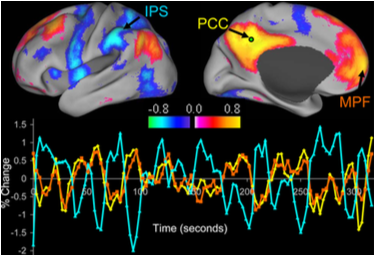
\includegraphics[scale=0.6]{default-mode}
\caption{\textit{Regions of a single subject's brain that are correlated (positive values) and anticorrelated (negative values) during resting  fixation in a functional MRI study. \textbf{Source: Fox et al (2005). \cite{DMN}}}}
\label{default-mode}
\end{figure}

After this discovery, other patterns of activities were found, leading to the definition of many resting state networks (RSNs) \cite{RNS}.

Different RSNs found by subsequent studies are visible in figure(\ref{resting-nws}).

\begin{figure}[!h]
\centering
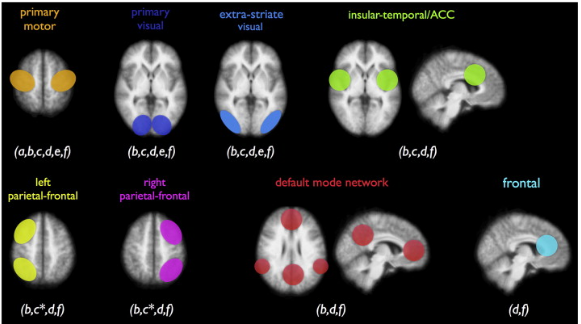
\includegraphics[scale=0.6]{resting-nws}
\caption{\textit{Different Resting State Networks found in literature and summarized by Van Den Heuvel et colleagues, 2010 \cite{RNS}}}
\label{resting-nws}
\end{figure}



The resting state can thus be defined as a cognitive state in which a subject is quietly awake and alert but does not engage in any specific cognitive or behavioural task \cite{Rest-NTW}.

\clearpage

\subsection{The Resting State in Brain Disease}

Most, if not all, physiological and psychiatric diseases have been found to have disrupted large-scale functional and/or structural properties.

This fact opens a wide array of possibilities as far as characterization, modelling and predictive studies are concerned for different types of disease.

Disorders like autism, schizophrenia and Alzheimer's disease have all been correlated to resting state network's alterations.
\vspace{5mm}

In example, Alzheimer's disesase diagnosed subjects have been found to have enhanced local network properties while having disrupted global properties with respect to non-diagnosed subjects \cite{ssa}.

Results of these type, based on the observations of altered topological properties of functional networks, are shown in fig.(\ref{ssa}).

\begin{figure}[!h]
\centering
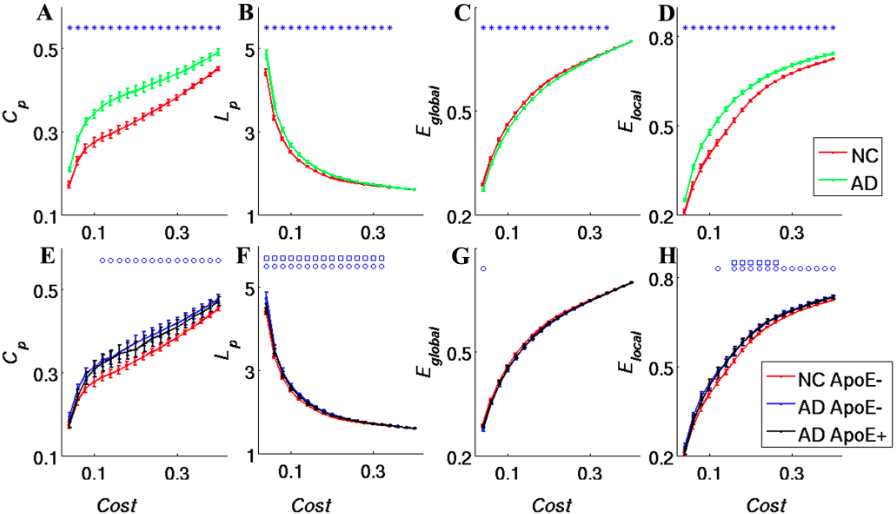
\includegraphics[scale=0.45]{ssa}
\caption{\textit{Change of network parameters as a function of connection density (Cost). Clustering coefficient (A), shortest path length (B), global efficiency (C) and local efficiency (D) of the AD (green line) and NC (red line) groups as a function of Cost. Clustering coefficient (E), shortest path length (F), global efficiency (G) and local efficiency (H) of the AD ApoE4+ (black line), AD ApoE4- (blue line) and NC ApoE4- (red line) groups as a function of Cost. The error bars correspond to the standard error of the mean. \textbf{Source: Xiaohu Zhao , Yong Liu et al. 2012 \cite{ssa}}}}
\label{ssa}
\end{figure}

\vspace{5mm}

We can see that \textit{clustering coefficients}, the \textit{shortest path length}, l\textit{ocal efficiency}, and \textit{connection density} are all enhanced in Alzheimer's disease diagnosed patients, whereas global efficiency is lower. 

As a matter of fact, $C_p$ is a measure of local network connectivity: it reflects the local efficiency and error tolerance of a network. 

Higher network clustering coefficients indicate more concentrated clustering of local connections and stronger local information processing capacity \cite{Rest-NTW}.

The $C_p$ of brain functional networks was found to be higher in Alzheimer's disease diagnosed patients, indicating that these patients have stronger local information processing capacity \cite{ssa}.

The average shortest path length ($L_p$) of a network reflects how the network connects internally. In brain networks, the shortest path ensures the effective integration and fast transmission of information between distant brain areas.
\vspace{5mm}

If the average shortest path of the brain functional networks in Alzheimer's disease diagnosed patients is significantly greater than that in non-diagnosed, it can be stated that the long distance information integration and transmission capacity of neurons is reduced in Alzheimers disease diagnosed patients.

Together with the lower global efficiency in Alzheimer's disease diagnosed subjects, these results may suggest that information transfer between brain regions is more difficult for these subjects \cite{ssa}.
\vspace{5mm}

Looking at which  brain's regions show a significant variation in topological functional newtork parameters, all of the typical default mode network can be identified as shown in fig.(\ref{rsz}).

\begin{figure}[!h]
\centering
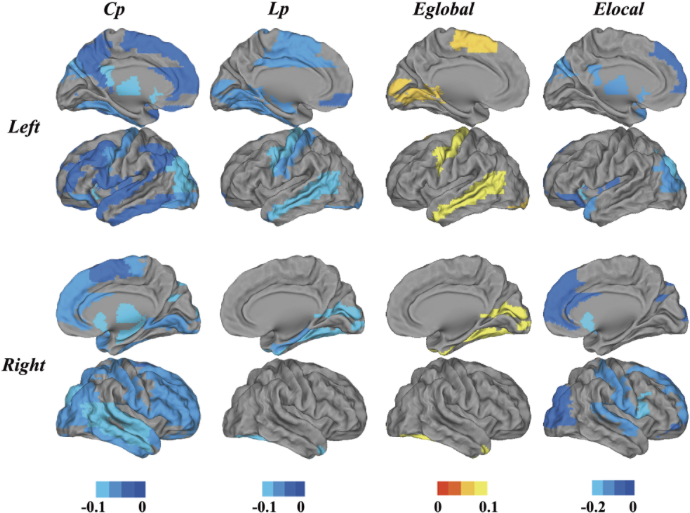
\includegraphics[scale=0.5]{rsz}
\caption{\textit{Surface rendering of the distribution of altered nodes at a connection density of 22\%.
Colored bars indicate differences in network properties between the NC and AD groups. Blue indicates regions showing an increase in the AD group but not the NCs. Yellow indicates regions showing a decrease in the AD group but not the NCs. In the AD group, the regions showing significant increases in $C_p$, $L_p$ and $E_{local}$ are widely distributed across the brain, especially in default mode network regions such as the ACC, PCC, MPFC, HIP and IPL. \textbf{Source: Xiaohu Zhao , Yong Liu et al. 2012 \cite{ssa}}}}
\label{rsz}
\end{figure}

This and many other studies relating to different types of disorders, show how investigating and modeling the default mode networks is of great importance in classification and preventive diagnosis methods implementation.

\clearpage

\section{Investigating the Resting State}

\subsection{The fMRI Technique}

The magnetic resonance imaging (MRI) is a non-invasive method largely used to obtain images of inner structures such as the human body.

The method is based on the magnetic properties of materials composed of nuclei having a non-zero spin.

Such nuclei, when placed in a magnetic  field $B_0$, arrange themselves over energetic levels according to the Boltzmann distribution, with the \textit{total magnetization} characterizing the order.
\vspace{5mm}

After introducing a perturbating pulse, which has to satisfy the \textit{resonance condition} of the system, the magnetization tends to realign itself with $B_0$ after a characteristic time, in which nuclei make transitions to set back the equilibrium.

The MRI follows the evolution of the system during the return to the equilibrium, obtaining informations about a system's properties and components via their characteristic time.
\vspace{5mm}

Let us consider an atomic nucleus with a non-zero total nuclear spin $\overrightarrow{I}$ ; the relation between the magnetic moment $\mu$ and the spin is:

\begin{equation}
\mu =\gamma  \hslash I
\end{equation}

where $\gamma$ is the magnetogyric ratio, which is tied to each nuclear isotope. Thus, the component along the $z$ direction of the magnetic moment is:

\begin{equation}
\mu_z =\gamma  \hslash m
\end{equation}

where $m$ can take one of the $2I+1$ values in the interval $[-I, I]$.

For $I=\frac{1}{2}$, an homogeneous applied external magnetic  field $B_0$ induces a splitting of the nuclear spin energy level:

\begin{equation}
\Delta E=\gamma  \hslash B_0
\end{equation}


Replacing the Planck-Einstein relation $\Delta E=h \nu$ in the latter equation, the \textit{Larmor resonance frequency} is obtained:

\begin{equation}
\nu_0=\frac{\gamma}{2\pi}B_0
\end{equation}

The corresponding pulsation $\omega_0$ is given by:

\begin{equation}
\omega_0=\gamma B_0
\end{equation}
\vspace{5mm}

The collective motion of a set of $N$ nuclei can then be observed by means of the \textit{total magnetization} $\overrightarrow{M}=N\langle \overrightarrow{\mu}\rangle$.

The evolution in time of the magnetization  of a set of nuclei placed a magnetic  field $B_0$ is:

\begin{equation}
\frac{d\overrightarrow{M}}{dt}=\gamma \overrightarrow{M} \times B_0
\end{equation}

The equation describes the precession of $\overrightarrow{M}$ around $\overrightarrow{B_0}$ at the angular velocity $\omega_0$, when $\overrightarrow{M}$ is not aligned with $\overrightarrow{B_0}$.

At the equilibrium, the total magnetization of a paramagnetic material placed in a magnetic field $\overrightarrow{B_0}$, shares the same direction of $\overrightarrow{B_0}$ as stated by \textit{Curie's law}:

\begin{equation}
\overrightarrow{M_0}=C\frac{\overrightarrow{B_0}}{T}
\end{equation}

where $T$ is the absolute temperature and $C$ is the \textit{Curie costant} that tied to material characteristics.

For the sake of simplicity $\overrightarrow{B_0}$ and $\overrightarrow{M_0}$ are considered aligned with the $z$ axis.
\vspace{5mm}

Applying a magnetic field  $\overrightarrow{B_1}$ orthogonal to  $\overrightarrow{B_0}$ with frequency $\nu_0$ causes the magnetization vector to move away from the $z$ axis; the angle between the $z$ axis and the new position of the magnetization vector depends on the duration of the radio frequency (RF)  field $\overrightarrow{B_1}$ applied, generated by a coil.

At the end of the pulse application, the spin precession on the transverse plane induces an oscillatory electromotive force in the coil by electromagnetic induction, thus originating a current in the probe.

The detectable signal is called \textit{Free Induction Decay} (FID), which has an oscillating trend with exponential decaying, and it is originated by photons in the radio-wave range emitted by the set of nuclei getting back to equilibrium.

After the RF pulse, the deacy of the NMR signal is analyzed in terms of two separate processes, the longitudinal one and the trasverse one, each with their own time constants.

The underlying process that leads the longitudinal component of the magnetization (along $z$) to reach its equilibrium value $M_0$, is the redistribution of nuclear spin populations according to the Boltzman distribution; such process takes place by energy exchanges between the nuclei and the surroundings.

The longitudinal component of the magnetization decreases in time, as defined by:

\begin{equation}
\frac{dM_z(t)}{dt}=-\frac{(M_z(t)-M_0)}{T_1}
\end{equation}

and thus:

\begin{equation}
M_z(t)=M_z(0)e^{-\frac{t}{T_1}}+ M_0(1-e^{-\frac{t}{T_1}})
\end{equation}

The underlying process that leads the trasverse component of the magnetization to reach its equilibrium value, i.e. zero, is the decoherence of the transverse nuclear spin magnetization. 

Random  fluctuations of the local magnetic  field lead to random variations in the instantaneous NMR precession frequency of different spins. 

As a result, the starting phase coherence of the nuclear spins is lost and the total $xy$ magnetization is null. 

The transverse component of the magnetization decays to zero in time according to:

\begin{equation}
\frac{dM_{xy}(t)}{dt}=-\frac{(M_{xy}(t)}{T_2}
\end{equation}

and thus:

\begin{equation}
M_{xy}(t)=M_{xy}(0)e^{-\frac{t}{T_2}}
\end{equation}

\begin{figure}[!h]
\centering
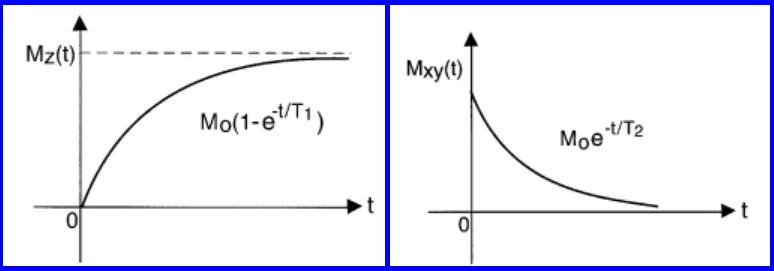
\includegraphics[scale=0.5]{relaxation}
\caption{\textit{ Evolution in time, after the RF pulse, of the longitudinal magnetization (left) and of the transverse magnetization (right) in the rotating frame. \textbf{Source: https://warwick.ac.uk/fac/sci/physics/research/condensedmatt}}}
\label{relaxation}
\end{figure}

\section{The BOLD Signal}

The \textit{Blood Oxygen Level Dependant} signal  is a measure of the amount of the oxygen contained in blood flowing towards neural regions.

To function properly, the brain needs energy in the form of \textit{Adenine-TriPhosphate} (ATP), which is in turn produced through a chemical reactions involving glucose and oxygen.

As neither glucose nor oxygen are stored in the brain by default, they need to be carried to the brain via circuclatory system. 

Oxygen is transported by \textit{haemoglobin}, in a chemical form  known as oxy-haemoglobin, in contrast to \textit{deoxy-haemoglobin}, the form haemoglobin assumes when it releases the transported oxygen.

These two molecular forms differ by their magnetic properties: oxy-haemoglobin is paramagnetic, whereas deoxy-haemoglobin is diamagnetic (fig.(\ref{haemo})).

\begin{figure}[!h]
\centering
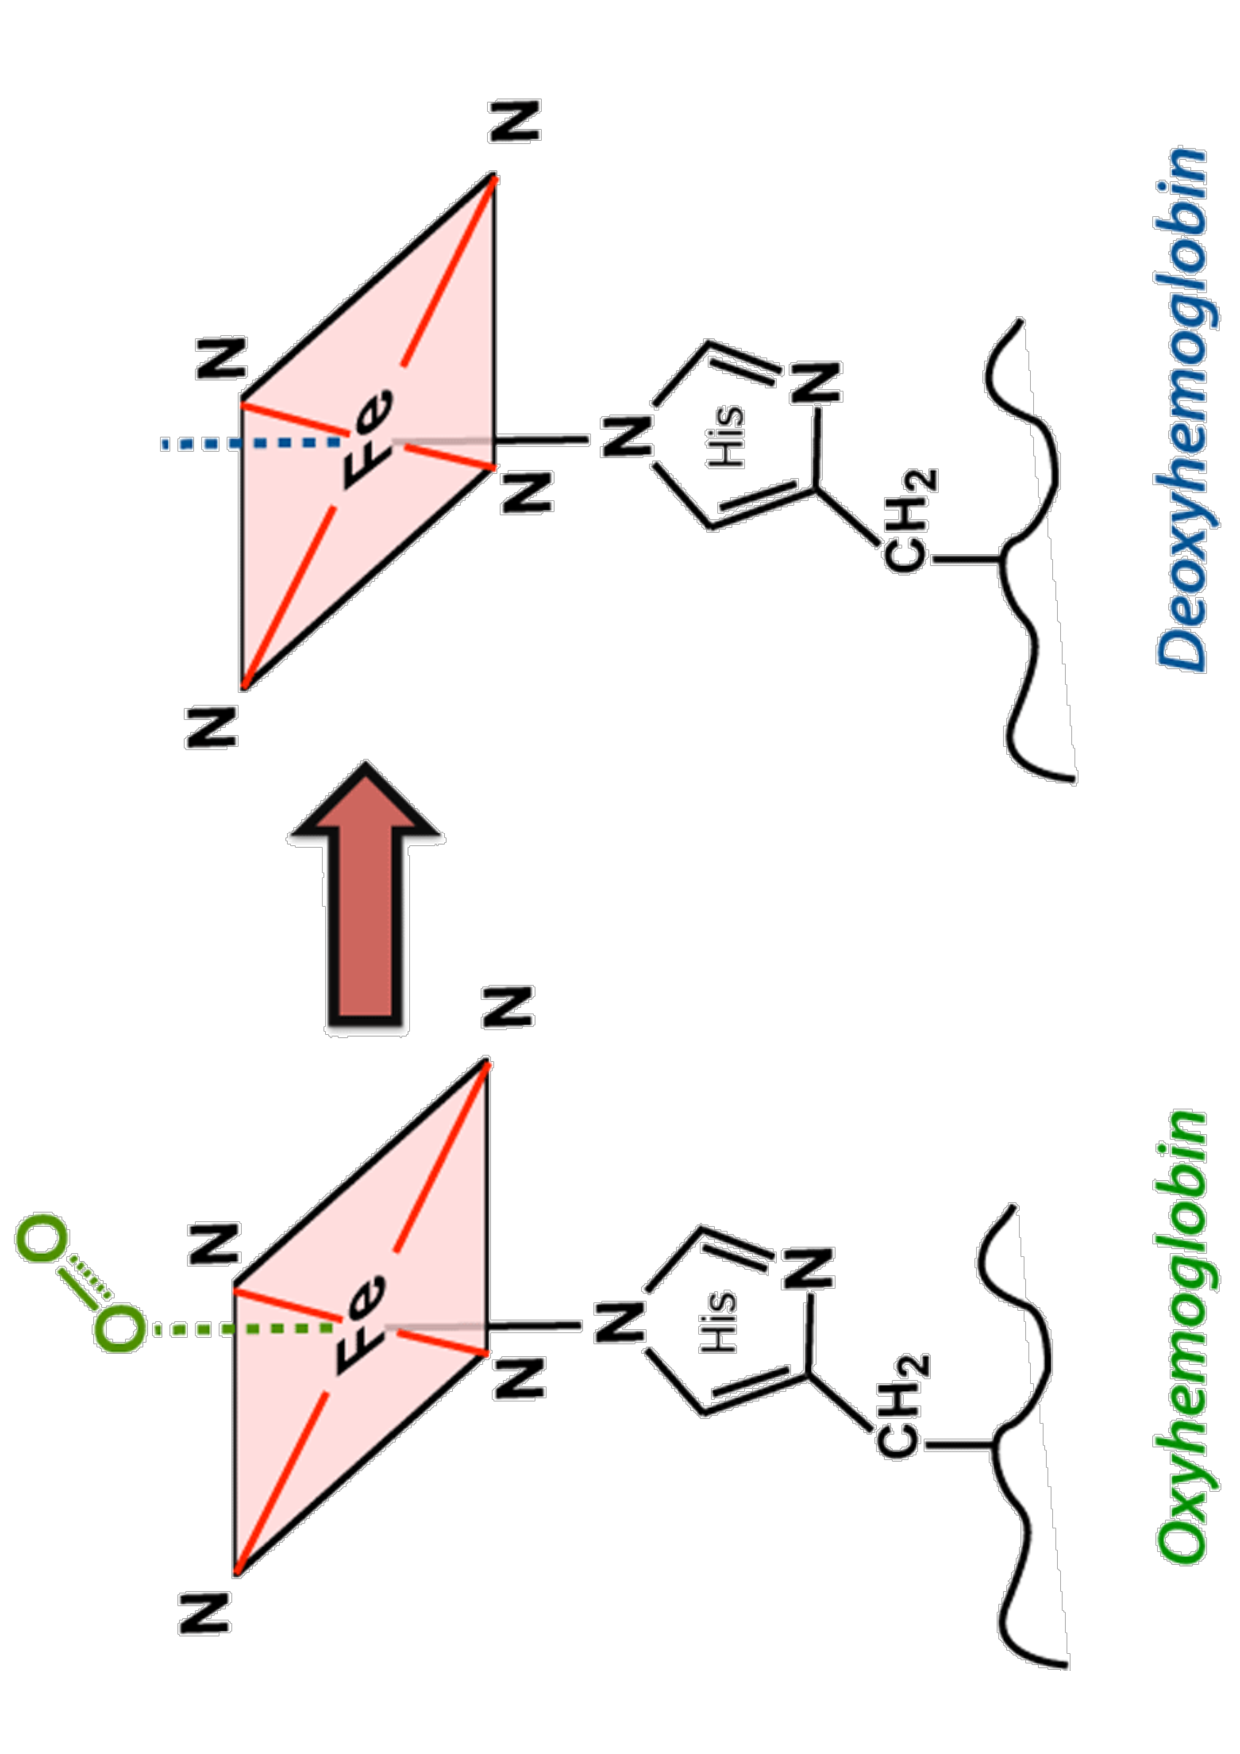
\includegraphics[scale=0.3, angle=270]{haemo}
\caption{\textit{ Deoxy-haemoglobin is trongly paramagnetic due to 4 unpaired electrons at each iron center. \textbf{Source: mriquestion.com/bold-contrast.html}}}
\label{haemo}
\end{figure}

When energy is required in a particular area, or in other terms a particular cerebral area is activated due to a given cognitive task, the amount of incoming oxygen (oxyhaemoglobin) is much higher than the oxygen being consumed to form ATP. 

As a result these areas show an increase in signal intensity.

More precisely, since the deoxyhemoglobin is paramagnetic, it is able to reduce the NMR signal in $T_2$ weighted images: indeed the rate of loss of proton spin phase coherence, measured through $T_2$, can be modulated by the presence of intravoxel deoxyhaemoglobin. On the contrary, being the oxyhemoglobin diamagnetic, it does not modify the NMR signal.
\vspace{5mm}

Thus, during the neural activation of a brain area, an higher incoming blood flux is observed with respect to the blood incoming during rest; in such area blood vessels expand and the transported oxygen rate is higher than oxygen consumed rate in burning glucose. 

Therefore, although paradoxical, in the active brain region the concentration of oxygenated blood increases, and the concentration of deoxygenated blood decreases with respect to the neighbour inactive brain areas. Such process is shown in fig.(\ref{bold}).

\begin{figure}[!h]
\centering
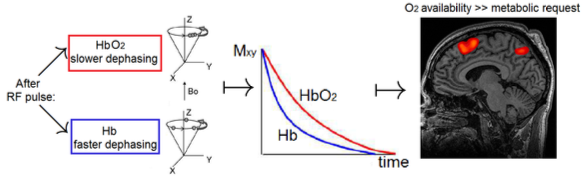
\includegraphics[scale=0.75]{bold}
\caption{\textit{BOLD signal formation process}}
\label{bold}
\end{figure}

It has to be pointed out, however, that the oxygen influx iunderlying the BOLD signal is not an immediate consequence of neural activity;they are rather parallel processes. 
\vspace{5mm}

In fact \textit{Glutamate-generated Calcium influx} releases many vasodilators. 

Blood flow is related more to local \textit{field potentials} than individual neurons spiking \cite{bold}; it can therefore be statede that the signal is increased over an area larger than the one with specific neuronal activity.
\vspace{5mm}

Given the high number of processes underlying global blood flow changes, a model tying BOLD signals to neural activity is required for those fMRI aplications whose goal is to observe and characterize neural processes.

The link between the the BOLD signal and the effective neural signal lies in the \textit{haemodynamic response function (HRF)}.

Formally, the BOLD signal can be interpreted as a \textit{convolution} between the actual neural signal and the HRF; the system's response to the stymulus is in ths way obtained.

If we take $N(t)$ as the neural activity signa and $h(t)$ as HDF we have:

\begin{equation}
B(t)=N(t)\ast h(t)=\int_0^t N(\tau)h(t-\tau)d\tau
\label{hdfconv}
\end{equation}

In order for eq.(\ref{hdfconv}) to be true, the assumption that the system's response is \textit{linear and time invariant} has to be made. We then define the neural signal as:

\begin{equation}
N(t)=\int_{t=0}^\infty \delta(t-\tau)n_{\tau}d\tau
\end{equation}

Given that the BOLD function is a function of neural activity $B(t) = f(N(t))$, linearity
implies that: 

\begin{equation}
f(\int_{t=0}^\infty \delta(t-\tau)n_{\tau}d\tau)=\int_{t=0}^\infty f[\delta(t-\tau)]n_{\tau}d\tau
\end{equation}

thus proving eq.(\ref{bold}).
\vspace{5mm}

Although many evidences indicate that BOLD signal is non-linear, deviations from linearity are often small and linearity assumptions are quite valid in many cases and apllications.

As the HRF depends on the ways oxygen is consumed when energy is required by neurons, it is complex to model as a function.

Even though eq.(\ref{bold}) holds true, most of the possible issues derive from $N(t)$ and $h(t)$ being both unknown in a large number of problems.

As a result, the HRF is often \textit{estimated} in order to be able to calculate the neural signal.

Many of the commonly used estimation methods rely upon recording the response to a given neural input, deconvolving eq.(\ref{bold}) while assuming a model for $N(t)$, or trying to guess the function and smooth it with some kind of parameter fitting.
\vspace{5mm}

Whichever the technique employed, one main feature of the HRF Must be taken into account for the consequences it induces on the BOLD signal $B(t)$: $h(t)$ has a low response, due to oxygen being quite slow (approximately 10 seconds) to reach its maximum value after neural activation.

As a consequence, for short and close neural impulses, the BOLD response does not have the chance to decrease, because of the convolution with the HRF. 

It thus can be stated that BOLD \textit{always smooths} the real underlying neural signal.

\section{Data Preprocessing}

The aim of data preprocessing is to reduce the statistical noise, in order to better extract the true signal.

This is most important for resting state analysis, given that there is no peak in the time series compared to the average value of the entire series. 

Looking at fig.(\ref{resting-nws}) in example, we can see that, as a matter of facts,changes in BOLD signal rarely exceed the $1\%$.
\vspace{5mm}

A resume of the most common preprocessing practices for fMRI studies is done in the following section.
\vspace{5mm}

\begin{itemize}
\item \textbf{Slice-timing correction}: All fMRI data are collected in \textit{slices}, which in turn contain arrays of voxels. 

The \textit{Repetition Time TR} is the time which separates the onsets of consecutive whole brain scans; thus is the time needed to collect data from all the brain voxels at a given point in time. 

This causes some problems to arise, i.e. not all the brain voxels in a given TR are acquired simultaneously: a TR time is needed to take all the slices between the first and the last. 

The bias is dependent on the order in which slices are taken. 

The most common approach to deal with such an issue is a form of \textit{temporal interpolation}, which can be linear, spline, or sinc. 

Linear interpolation is good when data do not vary much rapidly from one time acquisition to the other. This approach simply consists of estimating a continuous BOLD function from the discrete sampling; when using a linear function, a simple line is estimated between
two points, and the value at the point of interest is taken.

\item \textbf{Head motion correction}: It is probably the most important preprocessing step.

During task studies,  a movement of $5mm$ can increase activation values by a factor of $5$, and it can completely mix up signal from different voxels in resting state studies.

 All the corrections are based on the assumption that during movements the brain does not change size or shape; as a result, the only changes are due to rigid body movement. 
 
As a matter of fact, the movement can be characterised by \textit{six parameters}, 3 translational and 3 rotational, as described by classical mechanics. 
 
Voxels are defined by their position within the scanner,\textit{rather than by position within the subject’s brain}. 

To correct for this a \textit{rigid body registration} is performed.

\item \textbf{Normalization}: each individual presents morphologically different brains, with different global size and different local regions sizes  too. 

This leads to many problems while studying if a signal observed in one region is observed in the same region in another patient. 

Moreover, when performing group analyses, brains have to be overlapped, in order to increase the signal to noise ratio and the statistical significance of the analysis. 

However, if we overlap two significally different regions, the signal is quite likely to average out. 

Therefore, warping one subject’s structural image to a \textit{standard brain atlas} is a required step.

The most common reference system is the MNI space, developed by the Montreal Neurological Institute \cite{atlas}.

\item \textbf{Coregistration}: functional data have to be mapped onto structural data in order to as- sess the exact region the signal is coming from. 

These is not straightforward due to the two images being taken with different spatial resolutions. Given that functional images have to be taken within a few seconds, as a consequence of a speed-accuracy trade-off, they often have poor spatial resolution. 

Structural images, on the other hand, can take up to 10 minutes in order to be acquired if a precise mapping of every region is to be obtained.

This results in different voxel sizes: a typical fMRI voxel is $(3\times 3\times 3.5) mm$, whereas sMRI can have voxels with sizes down to $(0.86\time 0.86\times 0.89) mm$. 
After coregistration, however, structural resolution can be employed to improve functional resolution. 

Early methods aimed at identifying key landmarks in the two different images and then trying to align them, but given the scarce automation reliabiity of this process most methods now relies upon the minimisation of mutual information between histograms of the images.

\item \textbf{Data smoothing}: intensity values from individual voxel have an embedded component of noise. 

In order to reduce this noise spatial smoothing is needed; basically the intensity value of a voxel is replaced with a weighted average of the values of neighbouring voxels, through the convolution between the voxels and a function representing the neighbourhood known as \textit{kernel}. 

In this way, close voxels contribute much more than distant voxels. 

Other than increasing SNR, this process is useful since, as explained by the \textit{central limit theorem}, it allows the distribution of intensities to become normal thus helping the multiple comparison analysis in task studies.


\end{itemize}

\section{The Functional Connectivity Matrix}

One of the most common approaches in resting state studies gravitates around the notion of \textit{Functional Connectivity}.

Functional Connectivity is defined as \textit{the statistical association or dependency among two or more anatomically distinct time-series} \cite{connect}.
\vspace{5mm}

In FC analyses, there is no inference about coupling between regions; that is it does not tell \textit{how} regions are coupled.

In fact, it only tests some form of correlation against the null hypothesis.

FC is however useful to \textit{discover patterns} (which regions are coupled), and compare patterns, especially between groups.

In practice FC can be represented by a matrix whose entry $a_{ij}$ is a correlation between the intrinsic activity of neural source $i$ and neural source $j$.
\vspace{5mm}

Common examples of correlations measures computed on time-series data types are the \textit{cross-correlation} and \textit{cross-coherence} \cite{connect}.

Cross correlation between regions 1 and 2 with a time delay $t$ is given by:

\begin{equation}
R(t)= \frac{cov(1,2+t)}{\sqrt{var(s1)+var(s2+t)}}
\end{equation}

Cross-coherence can be defined as equivalent to cross-correlation but in the \textit{frequency domain}.

\chapter{The Wishart Distribution}

\section{Definition}

The \textit{wishart distribution} $ W_p(n, \Sigma)$ is a probability distribution of random nonnegative-definite $p\times p$ matrices that is used to model random covariance matrices.

The parameter $n$ is the number of degrees of freedom, and $\Sigma$ is a nonnegative-definite symmetric $p\times p$ matrix, called the \textit{scale matrix}.


\textit{Def.} Let $X_1...X_n$ be $N_p(0,\Sigma)$ distribuited vectors, forming a data matrix $p\times n$, $X=[X_1...X_n]$.
The distribution of  a $p\times p$, $M=XX'=\Sigma^n_{i=1}X_iX_i'$ \textit{random matrix}  is a Wishart distribution. \cite{AMS}

We have then by definition:

\begin{equation}
M\sim W_p(n, \Sigma)\sim\Sigma^n_{i=1}X_iX_i' \qquad X_i\sim N_p(0,\Sigma)   
\label{wsim}
\end{equation}


so that $M\sim W_p(n, \Sigma)$  is the distribution of a sum of $n$ rank-one matrices defined by independent normal $X_i \in R^p$ with $E(X)=0$ and $Cov(X)=\Sigma$.

In particular, it holds for the present case:

\begin{equation}
E(M)=nE(X_iX_i') = nCov(X_i) = n\Sigma
\end{equation}

\section{PDF Computation for Invertible $\Sigma$}

In general, any $X\sim N(\mu,\Sigma)$ can be represented as
\begin{equation}
X=\mu + AZ,\quad Z\sim N(0,I_p)
\end{equation}
so that
\begin{equation}
\Sigma= Cov(X) = A Cov(Z)A' = AA'
\label{covZ}
\end{equation}


The easiest way to find $ A$ in terms of $\Sigma$ is the LU-decomposition, which finds a unique lower diagonal matrix $A$ with $A_{ii} \geqslant 0 $ such that $AA' = \Sigma$.

Then by \ref{wsim} and \ref{covZ}, with $\mu=0$ we have:

\begin{equation}
W_p(n, \Sigma)\sim \sum_{i=1}^n(AZ_i)(AZ_i)'\sim A(\sum_{i=1}^nZ_iZ_i')A'\sim AW_p(n)A'
\end{equation}
where $Z_i\sim N(0, I_p)$ and $W_p(n)=W_p(I_p,n)$. 

Assuming that  $n\geq p$ and $\Sigma$ is invertible, the density of the random $p\times p $ matrix $M$ in \ref{wsim} can be written \footnote{\textit{Note: $\|\Sigma , N \| = det (\Sigma , M)$}} :

\begin{equation}
f(M, n, \Sigma)=\frac{1}{2^{\frac{np}{2}}\Gamma_p(\frac{n}{2})\|\Sigma\|^{\frac{n}{2}}}\|M\|^{\frac{n-p-1}{2}}exp[-\frac{1}{2}trace(\Sigma^{-1}M)]
\label{Wishart-pdf}
\end{equation} 

so that $f(M, n, \Sigma)=0$ unless $M$ is \textit{symmetric and positive-definite}. \cite{IMS}

Note that in \ref{Wishart-pdf} we define $\Gamma_p(\alpha)$ as the \textit{generalized gamma function} $\Gamma_p(\alpha)=\pi^\frac{p(p-1)}{4}\prod_{i=1}^p\Gamma(\frac{2\alpha+1-i}{2})$

\subsection{Visualizing the Wishart Distribution}

The Wishart distribution is a generalization to multiple dimensions of the \textit{chi-squared distribution}, or in the case of non-integer degrees of freedom, of the \textit{gamma distribution}.

We show as a proof in fig.\ref{Wish-chi2} that for a 1-dimensional and equal to 1 $\Sigma$ scale matrix, the Wishart distribution $W_1(n,1)$ collapses to the $\chi^2(n)$ distribution.

\begin{figure}[!h]
\centering
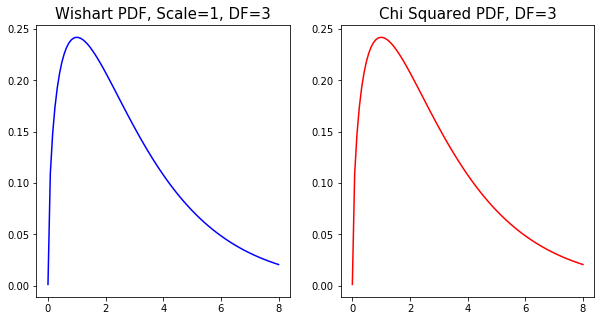
\includegraphics[scale=0.37]{wish-chi}
\caption{\textit{Monodimensional Wishart Distribution and $\chi^2(n)$ distribution comparison}}
\label{Wish-chi2}
\end{figure}

Save for this simple case, being the Wishart a distribution over matrices, it is a generally hard task to visualize it as a density function.

We can however sample from it and use the eigenvectors and eigenvalues of the resulting sampled matrix to define an ellipse.

An example of this technique is shown in fig.\ref{Wish-eig}. A set of five sampled matrices is drawn for each plot. While the parameter $n=2$ (\textit{degrees of freedom}) is the same for both the samplings shown, a different \textit{scale matrix} $\Sigma$ is used for each plot.

Note that for $\Sigma=I_2$ (left plot in fig.\ref{Wish-eig}) the sample would look \textit{on average} like circles.

\begin{figure}[!h]
\centering
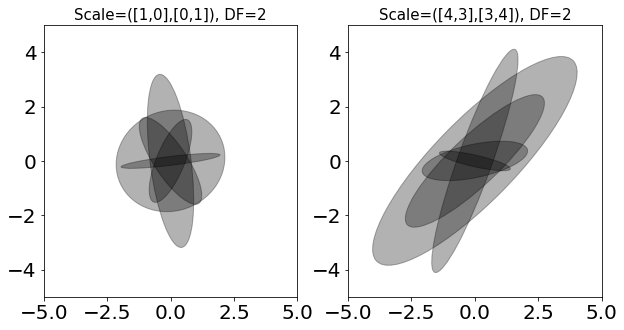
\includegraphics[scale=0.37]{wisheig-df2}
\caption{\textit{Plot of eigenvalue and eigenvectors defined ellipses, drawn from different scale matrix defined Wishart-sampled distribution. }}
\label{Wish-eig}
\end{figure}

\section{The Wishart Distribution in Bayesian Conjugate Prior Analysis}

An important use of the Wishart distribution is as a conjugate prior for \textit{multivariate normal sampling}. We now recall some basics concepts about Bayesian inference and prediction in order to show the application of the Wishart in those fields.

\subsection{Bayesian Inference and Priors Distributions}

The distinctive feature of the Bayesian approach underlies in its way of defining probability.

Probability is treated as \textit{belief} and not as \textit{frequency}, thus introducing a fundamental difference between the Bayesian and the \textit{frequentist} approach and shifting the goal toward the analysis and statement of a \textit{belief} \cite{SML}.
\\[12pt]
We can sum up the process of Bayesian inference as follows:
\begin{itemize}
\item A probability density called \textit{prior distribution} $\pi(\theta)$ is chosen, expressing the \textit{beliefs} about a parameter $\theta$ before any data are seen.
\item A statistical model $p(x\mid \theta)$ is chosen, which must reflect the beliefs about $x$ given $\theta$.
\item After observing the data $D_n=[X_1...X_n]$, the beliefs is updated and the \textit{posterior distribution} $p(\theta\mid D_n)$ is computed.
\end{itemize}

By Bayes' theorem the posterior distribution can be written as 

\begin{equation}
p(\theta\mid X_1...X_n)= \frac{p(X_1...X_n\mid \theta)\pi(\theta)}{p(X_1...X_n)}=\frac{L_n(\theta)\pi(\theta)}{c_n}\propto L_n(\theta)\pi(\theta)
\label{bayest}
\end{equation}

where $L_n(\theta)=\prod_{i=1}^n p(X_i\mid \theta)$ is the likelihood function and the \textit{normalizing constant} $c_n$ is defined as follows:

\begin{equation}
c_n=p(X_1...X_n)=\int p(X_1...X_n\mid \theta)\pi(\theta)d\theta=\int L_n(\theta)\pi(\theta)d\theta
\label{cnorm}
\end{equation}

the normalizing constant is also called the \textit{evidence}.

We now define the general properties of a \textit{conjugate prior}.

If, for a given problem, the posterior distribution $p(\theta\mid X_1...X_n)$ and the prior $\pi(\theta)$ belong to the same family of distribution, they're called \textit{conjugated distributions} and the prior is said to be a \textit{conjugate prior} for the given \textit{likelihood function} $L_n=p(X_1...X_n\mid \theta)$.

A classical example concerns the Gaussian Distribution: the Gaussian family is conjugate to itself (or self-conjugate) with respect to a Gaussian likelihood function: if the likelihood function is Gaussian, choosing a Gaussian prior over the mean will ensure that the posterior distribution is also Gaussian \cite{CBA}.

Considering the general problem of inferring a distribution for a parameter $\theta$ given some observations $D_n=[X_1...X_n]$ and referring to theorem \ref{bayest}, by which we let the likelihood function be considered fixed as it is usually well-determined from a statement of the data-generating process,  it is clear that different choices of the prior distribution $\pi(\theta)$ may make the integral in \ref{cnorm} more or less difficult to compute.
The product $L_n(\theta)\pi(\theta)$ will also be influenced, gaining the possibility to take one algebraic form or another.

If for certain choices of the prior the posterior has the same algebraic form as the prior, those choices are said to yield a \textit{conjugate prior}.

It is then possible to state that a conjugate prior is an algebraic convenience giving a closed-under-sampling-form expression for the posterior.

\subsection{The Wishart Conjugate Prior}

We now show how the Wishart Distribution is correlated to the\textit{Inverse Gamma Distribution} in a multidimensional setting, by  considering a Gaussian model with known mean $\mu$, so that the free parameter is the variance  $\sigma^2$, as in \cite{SML}.

The likelihood function is defined as follows:

\begin{equation}
p(X_1...X_n\mid \sigma^2)\propto (\sigma^2)^{-\frac{n}{2}}exp(-\frac{1}{2\sigma^2}n \overline{(X-\mu^2)}) , \qquad \overline{(X-\mu^2)}=\frac{1}{n}\sum_{i=1}^n(X_i-\mu)^2
\label{gausslike}
\end{equation}
\\[12pt]

The conjugate prior is an inverse Gamma distribution. Recall that $\theta$ has an inverse Gamma distribution with parameters $(\alpha,\beta)$   when $\frac{1}{\theta}\sim Gamma(\alpha,\beta)$.

The density is then bound to take the form 

\begin{equation}
\pi_{\alpha,\beta}(\theta)\propto \theta^{-(\alpha+1)}e^{-\frac{\beta}{\theta}}
\end{equation}

Using this prior, the posterior distribution of $\sigma^2$ is given by

\begin{equation}
p( \sigma^2 \mid X_1...X_n)\sim InvGamma(\alpha + \frac{n}{2}, \beta + \frac{n}{2} \overline{(X-\mu^2)})
\end{equation}

An alternative way of parameterization of the prior is given by the \textit{Inverse Scaled $\chi^2$ Distribution}, whose density is defined as

\begin{equation}
\pi_{\nu_0, \sigma_0^2}\propto \theta^{-(1+ \frac{n_0}{2})}exp(-\frac{\nu_0 \sigma_0^2}{2\theta})
\end{equation}

Under this kind of parameterization of the prior, the posterior takes the form

\begin{equation}
p(\sigma^2 \mid X_1...X_n)\sim ScaledInv\chi^2(\nu_0+n, \frac{\nu_0 \sigma_0^2}{\nu_0 + n} + \frac{n(X-\mu^2)}{\nu_0 + n})
\end{equation}

In the multidimensional setting, the inverse Wishart takes the place of the inverse Gamma.

It has already been stated that the Wishart distribution is a distribution over \textit{symmetric positive semi-definite} $d\times d$ matrices $W$. A more compact form of the density is given by

\begin{equation}
\pi_{\nu_0, S_0}(W)\propto \mid W\mid ^{\frac{(\nu_0-d-1)}{2}}exp(-\frac{1}{2}trace(S_0^{-1}W)), \qquad \mid W\mid=det(W)
\end{equation}

where the parameters are the degrees of freedom $\nu_0$ and the positive-definite \textit{scale matrix}
$S_0$.

If $W^{-1}\sim Wishart(\nu_0, S_0)$ we can then state that $W$ has an \textit{Inverse Wishart Distribution}, whose density has the form
\begin{equation}
\pi_{\nu_0, S_0}(W)\propto \mid W\mid ^{-\frac{(\nu_0+d+1)}{2}}exp(-\frac{1}{2}trace(S_0W^{-1})), \qquad \mid W\mid=det(W)
\end{equation}

Let $X_1...X_n$ be $N(0,\Sigma)$ distributed observed data. Then an inverse Wishart prior multiplying the likelihood $p(X_1...X_n\mid \Sigma)$ yields

\begin{equation}
\begin{aligned}
p(X_1...X_n\mid \Sigma)\pi_{\nu_0, S_0}(\Sigma)\propto \\[10pt]
 \mid\Sigma \mid ^{-\frac{n}{2}}exp(-\frac{n}{2}trace(\overline{S} \Sigma^{-1}) \mid \Sigma\mid ^{-\frac{(\nu_0+d+1)}{2}}exp(-\frac{1}{2}trace(S_0\Sigma^{-1})) \\[10pt]  
=  \mid \Sigma\mid ^{-\frac{(\nu_0+d+n+1)}{2}}exp(-\frac{1}{2}trace((n\overline{S}+S_0)\Sigma^{-1}))
\end{aligned}
\end{equation}

where $\overline{S}$ is the \textit{empirical covariance} $\overline{S}=\frac{1}{n}\sum_{i=1}
^nX_iX_i^T$.

Thus, a posterior with the form

\begin{equation}
p(\Sigma\mid X_1...X_n)\sim InvWishart(\nu_0+n, n\overline{S}+S_0)
\end{equation}

is obtained.

Analogally, it can be stated that for the inverse covariance (\textit{precision}) matrix $\Sigma^{-1}$ the conjugate prior is a Wishart distribution.

\chapter{The WISDoM Multiple Order Classification}

In this section, the classification method implemented and used on the ADNI2 and ABIDE databases is described, both in an analytical and technical way.
\vspace{5mm}

The Wishart Distributed Matrices Multiple Order Classification is a method that allows both classification and \textit{feature selection} for any classification problem whose elements can be tied to a \textit{symmetric positive-definite} matrix representation (i.e. covariance and correlation matrices).

 The \textit{"distance"} used to train the classifier is defined as well as the \textit{feature transformation} undergone by the each of the subject analyzed.

The general pipeline and the validation pipeline are then discussed while also introducing an example of possible parallelization for performance enhancing.

\section{Wishart Sampling}

Considering what has been said in the last section, using the Wishart distribution to model and sample the elements of a wide range of problems follows naturally.

As a matter of fact, every calssification problem whose elements take the form of \textit{symmetric positive-definite} matrices can be approached with the method we are about to discuss.

The main idea for the \textit{WISDoM Classifier} is to use the \textit{free parameters} of the Wishart distribution (the scale matrix $S_0$ and the number $n$ of the degree of freedom, as shown in \ref{Wishart-pdf}) to compute an estimation of the distribution for a certain class of elements, and then assign a single element to a given class by computing some sort of distance between the element being analyzed and the classes.

Furhermore, if we assume that the matrices are somehow representative of the \textit{features} of the system studied (i.e. covariance  matrices might be taken into account), a score can be assigned to each feature by estimating the weight of said feature in terms of \textit{Log Likelihood Ratio}.

In other words, a score can be assigned to each feature by analyzing the variation in terms of \textit{LogLikelihood} caused by the deletion of it. 

If the deletion of a feature causes significant increase (or decrease) in the \textit{LogLikelihood} computed with respect to the \textit{estimated distributions} for the classes, it can be stated that said feature is highly representative of the system analyzed.

It is now clear that the simplest usable objects to estimate the distribution for a class and to represent its elements is the \textit{covariance  matrix}. Further proofs for this statement will be given later on.

Thus, the aim of the WISDoM classifier is not only to assign a given element to the optimal class, but also to identify the features with the highest \textit{"weights"} in the decision process.

\subsection{Computing the Estimated Distribution}

Let us briefly recall the parametrization of the Wishart Distribution in order to clearly define the application conditions for classification problems.

Let $X_1...X_n$ be independent $N_p(0,\Sigma)$ distributed vectors, forming a data matrix $p\times n$, $X=[X_1...X_n]$.
The distribution of  a $p\times p$, $M=XX'=\Sigma^n_{i=1}X_iX_i'$ \textit{random matrix}  is a Wishart distribution with parameters $W_p (n, S_0 )$. In the previous chapter (\ref{Wishart-pdf}) it has been proved that for normal distributed data, for $S_0=\Sigma$, a distribution of \textit{random covariance matrices} is obtained.

In a similar fashion, if a good choice for the scale matrix $S_0$ is made for a given class, a representative distribution for the class can be estimated and samples can be drawn from it.

\textit{Covariance matrices} are a good choice, although not limiting as long as the matrices are symmetric and positive-definite, both for the way they represent a system and for the property that \textit{the mean of a set of covariance matrices is a covariance matrix}. 

If each element of a given class $C$ is represented by a covariance matrix $\Sigma$ of its features, this property allows us to estimate a distribution for the class by choosing 
\begin{equation}
S_0=\hat{\Sigma}_C=\frac{1}{N}\sum_{i=1}^N \Sigma_i
\label{Class-Scale}
\end{equation}


The other necessary parameter for the estimation is the \textit{degrees of freedom n}.

Assume that an $X_i=(x_1, ..., x_p)$ vector of $p$ features is associated to each element $i$ of a given class, while having $n$ observation of said vector. The covariance matrix $\Sigma_i$ computed over the $n$ observations will represent the "interactions" between the features of element $i$.

The degrees of freedom  $n$ of the Wishart distribution are then given by the number of times $X_i$ is observed.

Let us introduce an example tied to \textit{functional MR brain imaging } in order to further clarify the concepts being introduced. 

An image of patient $i$'s brain is acquired; as usual these images are divided in a certain number $p$ of zones (voxel, pixel etc.), each zone being sampled $n$ times over a given time interval in order to observe a certain type of brain activity and functionality.

It is now clear that the features contained in vector $X_i=(x_1,..,x_p)$ associated to patient $i$ are indeed the zones chosen to divide $i$'s brain image, each zone having been sampled $n$ times during an acquisition interval.

The correlation $p \times p$ matrix $\Sigma_i$ computed for $i$'s observation is then representative of the functional correlation between the $p$ zones of $i$'s brain.

Repeating this procedure for $N$ patients belonging to a known class $C$ (i.e. a diagnostic group) and computing the $\hat{\Sigma}_C$ scale matrix for the class as stated before, will allow us to estimate a wishart distribution for that class correlation matrices and draw samples from it.

\vspace{5mm}

The module used for Wishart generation and sampling by the WISDoM calssifier is the \textit{SciPy.Stats.Wishart} module of the \textit{SciPy} Python3.6 library.

Further details on the generation and sampling algorithm used  by the module can be found in \cite{WishGen}.

Some  samples drawn from Wishart distributions computed with different  $5 \times 5$ scale matrices and degrees of freedom are shown in fig.\ref{randmatr}.

\clearpage

\begin{figure}[!h]
\centering
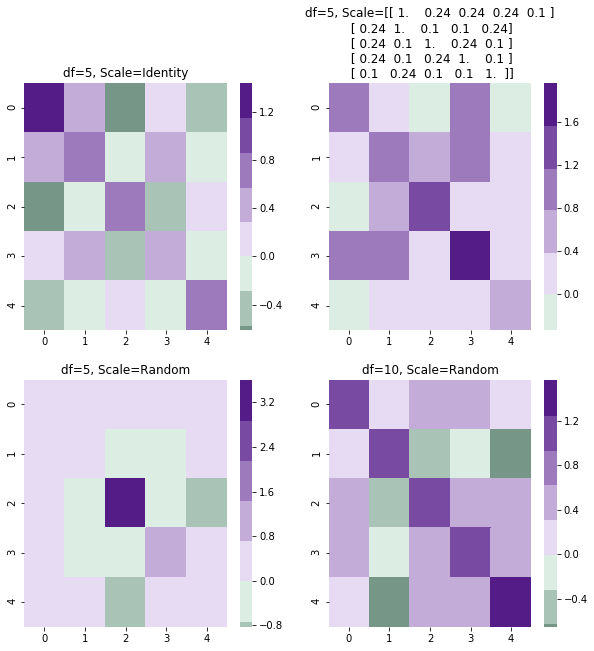
\includegraphics[scale=0.5]{randmatr}
\caption{\textit{Various sampling from different wishart distribution. A diverging heatmap has been chosen to visualize the values of each sample's elements.}}
\label{randmatr}
\end{figure}

\section{Log-Likelihood Ratio Distance}

After the definition of the role of the Wishart distribution in symmetric positive definite matrices' modeling, it is necessary to define some sort of distance between the estimated distribution for a class $C$ and its hypotetical elements.

As stated before, this will be done in terms of both entire matrices and \textit{single features}, in order to achieve optimal classification and exract information about a system's most meaningful components.

\subsection{Complete Matrix Distance}

The scoring system used by the WISDoM Classifier relies on the \textit{logpdf} function from the \textit{SciPy.Stats.Wishart} module in order to compute the LogLikelihood of a matrix $\Sigma_i$ with respect to the Wishart distribution estimated for a class $C$, using $\hat{\Sigma}_C$ as the scale marix.

If a problem concering two given classes $C_A$ and $C_B$ is taken into account, the score assigned to each $\Sigma_i$ upon which the classification decision is based, can be defined as follows:

\begin{equation}
score_{i}= logP_{W}(\Sigma_{i}\mid n, \hat{\Sigma}_{A})-logP_{W}(\Sigma_{i}\mid n,\hat{\Sigma}_{B})
\label{pdf-score}
\end{equation}

Where $\hat{\Sigma}_{A,B}$ are the scale matrix computed for the classes $A,B$ and $ logP_{W}(\Sigma_{i}\mid n, \hat{\Sigma}_{A,B})$ can be seen as the logarithm of the probability of $\Sigma_i$ belonging to the Wishart distribution estimated for one of the two classes $A,B$.

\subsection{Single Feature Distance and Multiple Order Reduction}

The aim of the WISDoM classifier is to further increase the informations obtained about the system's features during the classification.

To do this it is then necessary to introduce some matemathical properties of the symmetric positive deifnite matrices, upon which the method relies.

It will be shown that it is indeed possible to access different orders of information by scaling a matrix $A$ to its \textit{principal submatrices}.

\vspace{5mm}

\textbf{Def.} \textit{Let $A$ be an $n \times n$ matrix. A $k \times k$ submatrix of $A$ formed by deleting $n-k$ rows of $A$, and the same $n-k$ columns of $A$, is called principal submatrix of $A$. The determinant of a principal submatrix of $A$ is called a principal minor of $A$.}

\vspace{5mm}

Note that the definition does not specify which $n-k$ rows and columns to delete, only that their indices must be the same.

Let us introduce a $3 \times 3$ example.

For a general matrix $A_{3\times 3}$ 

\begin{equation}
A=
\begin{bmatrix}
         a_{11} & a_{12} & a_{13} \\
    	    a_{21} & a_{22} & a_{23} \\ 
	    a_{31} & a_{32} & a_{33}  
\end{bmatrix}
\end{equation}

\vspace{5mm}

there are three \textit{first order principal minors}:

\begin{itemize}
\item $\mid a_{11}\mid$ formed by deleting the last two rows and columns
\item $\mid a_{22}\mid$ formed by deleting the first and third rows and columns
\item $\mid a_{33}\mid$ formed by deleting the first two rows and columns

\end{itemize}

There are three \textit{second order principal minors}:

\begin{itemize}
\item 
$\mid\begin{bmatrix}
         a_{11} & a_{12}  \\
    	    a_{21} & a_{22}  \\ 
\end{bmatrix}\mid$ formed by deleting column 3 and row 3

\item
$\mid\begin{bmatrix}
         a_{11}  & a_{13} \\
	    a_{31}  & a_{33}  
\end{bmatrix}\mid$ formed by deleting column 2 and row 2

\item
$\mid\begin{bmatrix}
         a_{22} & a_{23} \\ 
	     a_{32} & a_{33}  
\end{bmatrix}\mid$ formed by deleting column 1 and row 1

\end{itemize}

There's one \textit{third order principal minor}, namely $\mid A\mid$.

\vspace{5mm}

For the sake of completion, we also recall the following definition.

\textbf{Def.} \textit{Let $A$ by an $n\times n$ matrix. The $k^{th}$ order principal sub-matrix of $A$ obtained by deleting the \textbf{last} $n-k$ rows and columns of $A$ is called the $k^{th}$ order \textbf{leading principal submatrix} of $A$, and its determinant is called the  $k^{t}h$ \textbf{order leading principal minor} of A.}
\vspace{5mm}

An imporant property for the principal submatrices of a symmetric positive definite matrix is that \textit{any $(n-k)\times (n-k)$ partition is also symmetric and positive definite.}

It is now clear that such properties can be used to reduce both a class scale matrix $\hat{\Sigma}_C$ and any $\Sigma_i$ matrix, in order to study its deviation from a class's estimated Wishart distribution derived from the deletion of one of its components (the features conatined in vector $X_i=(x_1,...,x_p)$ from which the matrix $\Sigma_{i,p\times p}$ is computed).

Iterating this process over all the features, or in other terms analyzing all of the $(p-1)\times (p-1)$ principal submatrices of $\Sigma_i$ and $\hat{\Sigma}_C$, will allow us to assign a score to each feature, representing its weight in the decision for $\Sigma_{i}$ to be assigned to one class or another.

Note that for such an order of principal submatrices, the process will reduce the $\Sigma_{i,p \times p}$ matrix to a \textit{score vector} of length $p$ for each element $i$ undergoing the classification.

Let us now introduce the following notation in order to define the score assigned for each of the $x_p$ features of the vector $X_i=(x_1...,x_p)$.

Let $\Sigma_j$ be a principal submatrix of order $(p-1)$, of the matrix $\Sigma$ computed on the observation of $X_i=(x_1,...,x_p)$ for subject $i$, \textit{obtained by the deletion of the $j^{th}$ row and the $j^{th}$ column}, with $ 1\leq j\leq p$.
\vspace{5mm}

Let  $\hat{\Sigma}_{Cj}$  be a principal submatrix of order $(p-1)$, of the matrix $\hat{\Sigma}_C$ computed for the class $C$ \textit{obtained by the deletion of the $j^{th}$ row and the $j^{th}$ column}, with $ 1\leq j\leq p$.
\vspace{5mm}

The score assigned to each feature of $X_i=(x_1,...,x_p)$ is then given by eq.(\ref{JSscore}).

\begin{equation}
Score_j(C)=\Delta logP_{Wj}(C)=logP_W(\Sigma, n \mid \hat{\Sigma}_C,n)-logP_W(\Sigma_j, n \mid \hat{\Sigma}_{Cj},n)
\label{JSscore}
\end{equation}
\vspace{5mm}

In other terms, each partition $\Sigma_j$ represents the matrix $\Sigma$ without the elements tied to feature $x_j$ (the elements in row $j$ and column $j$ of $\Sigma$). Computing the variation in terms of log-likehood  between the estimated wishart distribution for the class and the estimated wishart distribution for the class without component $j$, allows us to gain informations about which feature weighs more on both subject $i$'s cassification and the general system structure.

Note that this kind of scoring is \textit{class-dependent}. Computing this score vector with respect to all the classes $C_1..C_n$ of a given problem and performing  some sort of score ratio will allow the subject $i$, after a suitable \textit{training},  to be assigned to the most likely of the classes while retaining informations on which features are the most determinant, decision wise.
\vspace{5mm}

Let us introduce a \textit{2-classes} example in order to show how this kind of result might be obtained.

Let $C_1$ and $C_2$ be the two classes of a given problem. 

Let a set of $N$ matrices $\Sigma_i$ be a set of correlation matrices computed for $N$ subjects $i$ whose class is known. 

Let $\hat{\Sigma}_{C1}$ and $\hat{\Sigma}_{C2}$ be  the scale matrices computed as seen in eq.(\ref{Class-Scale}), used to estimate the Whishart distribution for each one of the two classes $C_1$ and $C_2$, and  $\hat{\Sigma}_{C1j}$ and $\hat{\Sigma}_{C2j}$ their $(p-1)$ order partitions, as in eq.(\ref{JSscore}).

If from each matrix $\Sigma_i$ the score vector is computed as in eq.(\ref{JSscore}) with respect to each one of the two classes $C_1,C_2$, an \textit{inter-class log-likelihood ratio vector} can be obtained by assigning to each feature a score defined as follows:

\begin{equation}
Ratio_j=\Delta logP_{Wj}(C_1)-\Delta logP_{Wj}(C_2)
\label{JRatio}
\end{equation}

Training a classificator on a set of $N$ subjects whose classes are known, after each matrix $\Sigma_i$ (and as a consequence each feature vector $X_i$) has undergone the transformations defined in eq.(\ref{JSscore}) and (\ref{JRatio}), yields a significant improvement in performance for certain classes of problems, as it will be shown later.

A new subject will be, as a matter of fact, classified according to its \textit{transformed ratio vector} given by eq.(\ref{JRatio}), thus simultanesously retaining information about its class's most significant features: \textit{the score assigned to each feature is a measure of how much the deletion of said feature weighs, in terms of log-likelihood variation, on the decision to assign each matrix $\Sigma_i$ to one class or another.}
\vspace{5mm}

The entire process can be seen as a \textit{feature transformation}, which leads to a \textit{feature selection}, whose effect is, for certain types of problems, to enhance the classification performance.

\subsection{Generalizing to $(p-n)$ Order Transformations}
As seen in the last section, transforming all the $(p-1) \times (p-1)$ principal submatrices of $\Sigma_i$ by eq.(\ref{JSscore}), yields a vector of score of length $p$ for each element $i$.

Anyway, for any $n<p$, a number of principal submatrices of $\Sigma_i$ can be obtained.

These kind of submatrices can be used to gain informations about the weight of $n$ simoultaneously deleted features on the system structure and classification.

Let us introduce an example for $(p-2)$ order submatrices.
\vspace{5mm}

Let $\Sigma_{jk}$ be a principal submatrix of order $(p-2)$, of the matrix $\Sigma_i$ computed on the observation of $X_i=(x_1,...,x_p)$ for subject $i$, \textit{obtained by the deletion of the $j^{th}$ row and the $j^{th}$ column and the $k^{th}$ row and the $k^{th}$ column }, with $ 1\leq j,k\leq p$.
\vspace{5mm}

Let  $\hat{\Sigma}_{Cjk}$  be a principal submatrix of order $(p-2)$, of the matrix $\hat{\Sigma}_{Cjk}$ computed for the class $C$ \textit{obtained by the deletion of the $j^{th}$ row and the $j^{th}$ column and the $k^{th}$ row and the $k^{th}$ column }, with $ 1\leq j,k\leq p$.
\vspace{5mm}

Then, eq.(\ref{JSscore}) becomes:

\begin{equation}
Score_{jk}(C)=\Delta logP_{Wjk}(C)=logP_W(\Sigma, n \mid \hat{\Sigma}_C,n)-logP_W(\Sigma_{jk}, n \mid \hat{\Sigma}_{Cjk},n)
\label{JKSscore}
\end{equation}
\vspace{5mm}

in this case, a score is assigned to each coupling of the features $j,k$, and transformation (\ref{JKSscore}) will yield not a vector, but a $p\times p$ matrix with diagonal elements equals to the scores obtained by (\ref{JSscore}), being the iteration with $j=k$ the coupling the $j^{th}$ feature with itself. 

Non-diagonal elements represent the score of the coupling of feature $j$ with feature $k$.

\section{Pipeline}

In this section we discuss each step of the feature transformation and classification process.

Given the recursive nature of the method just described, a crucial issue concerning computational time is the strong dependence between it and the analyzed matrix size.

A rough visualization of the entity of  such a dependence can be found in fig.(\ref{timevsize})

\begin{figure}[!h]
\centering
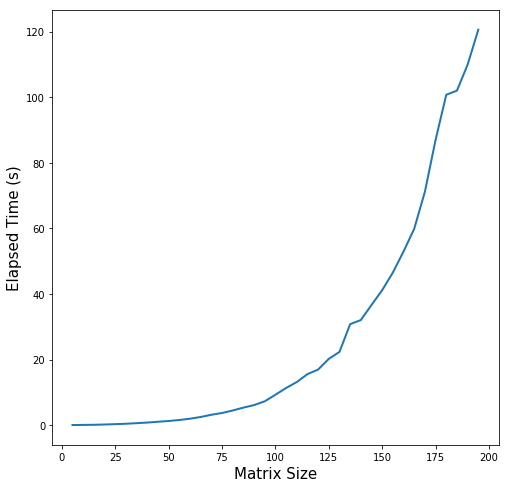
\includegraphics[scale=0.42]{RC2-timeVsize}
\caption{\textit{Matrix Size dependence for $(p-2)$ order transformations.}}
\label{timevsize}
\end{figure}

Iterating the $(p-1)$ order transformation described in eq.(\ref{JSscore}) over a large $N$ of observations of size $	p \times p$ of a given database, while introducing some kind of \textit{cross-validation} routine may lead to abysmal computational time-wise performances.
\vspace{5mm}

A possible solution to this problem is to introduce a high level of automatization for each step, followed by the indroduction of a highly parallelizable overall structure of the pipeline.

\subsection{The Snakemake Environment}

The main tool used to achieve such results is the \textit{ Snakemake Workflow Management System}, described in \cite{SnakeMake}, a Python-based interface created to build reproducible and scalable data analyses and machine-learning routines.

To briefly some up the the advantages of using such tools and structures, the \textit{Snakemake Workflow} can be described as rules that denote how to create output files from input files. The workflow is implied by dependencies between the rules that arise from one rule needing an output file of another as an input file \cite{SnakeMake}.

A rule definition specifies :

\begin{itemize}
\item \textit{a name}, used by the main rule instance \textit{rule all} and main execution environment for identification
\item \textit{any number of input and output files}; tipically one rule's output is another rule input, linking the rules alla the way up to main rule instance.
\item  \textit{either a shell command or Python code}; containing the creation of the output from the input
\end{itemize} 

Input and output files may contain multiple named \textit{wildcards}, whose values are inferred automatically from the files desired by the user.
\vspace{5mm}

To further clarify the role of the wildcards, let us introduce a brief example.

Let's say that our aim is to train a classifier over two classes of elements $C_1,C_2$. The training part of the database is then divided in two files, each one containing the name of its elements' class in the filename.

Setting a rule to load these files while expecting a wildcard tied to the class name in the filename, will allow the entire set of rules of the pipeline to be executed automatically for class $C_1$ and class $C_2$.

Considering this example, the real power of the parallelization capabilities offered by the Snakemake environment are quite clear.

With a simple syntax, looking at the example just proposed, each one of two \textit{cores} of a server where our hypothetical pipeline is running can be set to work indipendently on each subset of data belonging to class $C_1$ or class $C_2$.

Building a pipeline whose rules are easily iterable over a set of different \textit{wildcards} will lead to natural and efficient parallelization and automation.

\subsection{The WISDoM Pipeline}

\begin{figure}[!h]
\centering
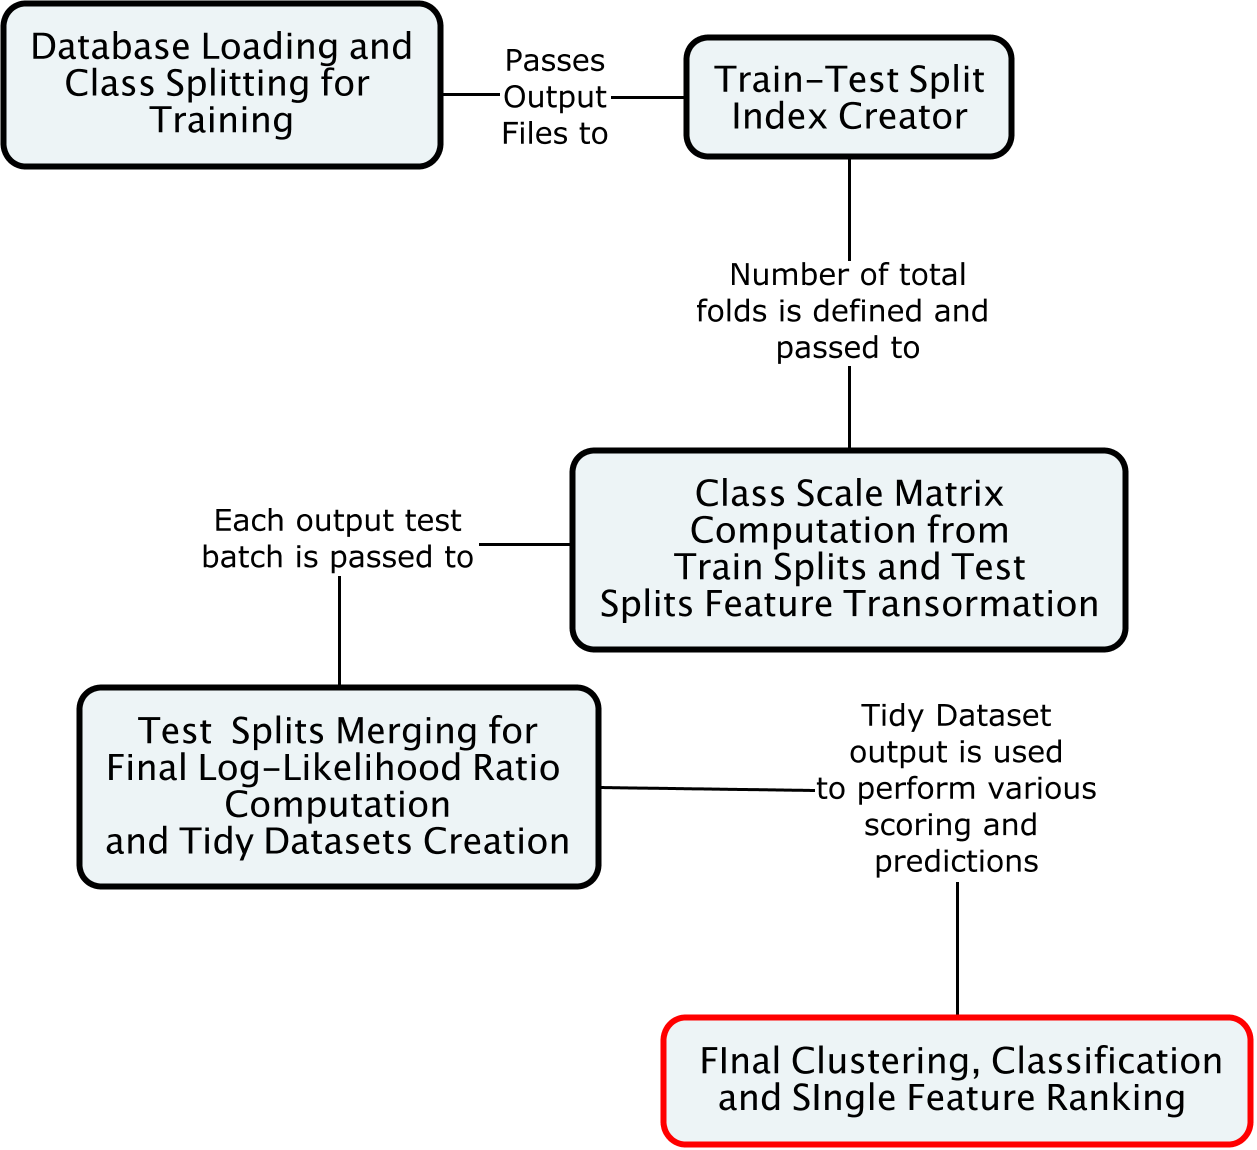
\includegraphics[scale=0.3]{General-Pipeline}
\caption{\textit{General pipeline workflow.}}
\label{gpipe}
\end{figure}

In figure (\ref{gpipe}) the main steps required by the WISDoM Multiple Order Classification are reported.

We will now go through each step in detail in order to show how \textit{train and test splitting} are interpreted for the WISDoM pipeline.

\begin{itemize}
\item \textbf{Database loading and class splitting}\\
\textit{rules: case\_wrap, seqs\_store} ; in this section of the pipeline, data are loaded and divided into the classes defined by the wildcards and main rule instance's inputs. An info sheet containing the classification labels for each observation is needed as an \textit{input} for this step. 

In order to achieve fast reading/writing perfomances for big data, the matrices are stored as the sequence of elements belonging to the upper triangle for each matrix (in \textit{.hdf} format). Being symmetric, the entire matrix can be easily reconstructed when needed. At this step, the files containing observations for each class are created.

\item \textbf{Train-Test split index creator}\\
\textit{rules: split\_gen, tt\_gen}; in this section of the pipeline, each file containing one class's observations is divided into train-test batches. The total number of train-test folds is defined by wildcards and main rule instance's inputs. 

First, each dataset is divided into sections, then each section is further splitted intoa number of user-specified  train-test folds.

\item \textbf{Class Scale Matrix computation and feature transformation}\\
\textit{rules: map\_gen}; this is the core section of the pipeline, where the features are transformed according to eq.(\ref{JSscore}).

Train-test split files for each class are passed as inputs; the train sets of each batch are used to compute the scale matrix $\hat{\Sigma}_C$ as in eq.(\ref{Class-Scale}). The estimated Wishart for the class is then computed and the features of each test-set element are transformed.

In order to compute the Ratio described in eq.(\ref{JRatio}), the above process is repeated for each class with respect to each other. A map containing each transformed feature in term of \textit{quantiles} is also created.

\item \textbf{Test splits merging and tidy datasets creation}\\
\textit{rules: t\_join, q\_join}; in the final step of the pipeline, all of the transformed feature test batches are merged into tidy datasets. This type of data sturcture will allow an easy computation of the ratio in eq.(\ref{JRatio}) for each feature; furhtemore, once such dataset is obtained, evertything needed for the transformed observations to undergo any classification pipeline and/or model selection is ready.
\end{itemize}

A graphic representation of the plan of rules execution can be obtained by using a \textit{directed acyclic graph} (DAG), as shown in figure (\ref{dag}).

\begin{figure}[!h]
\centering
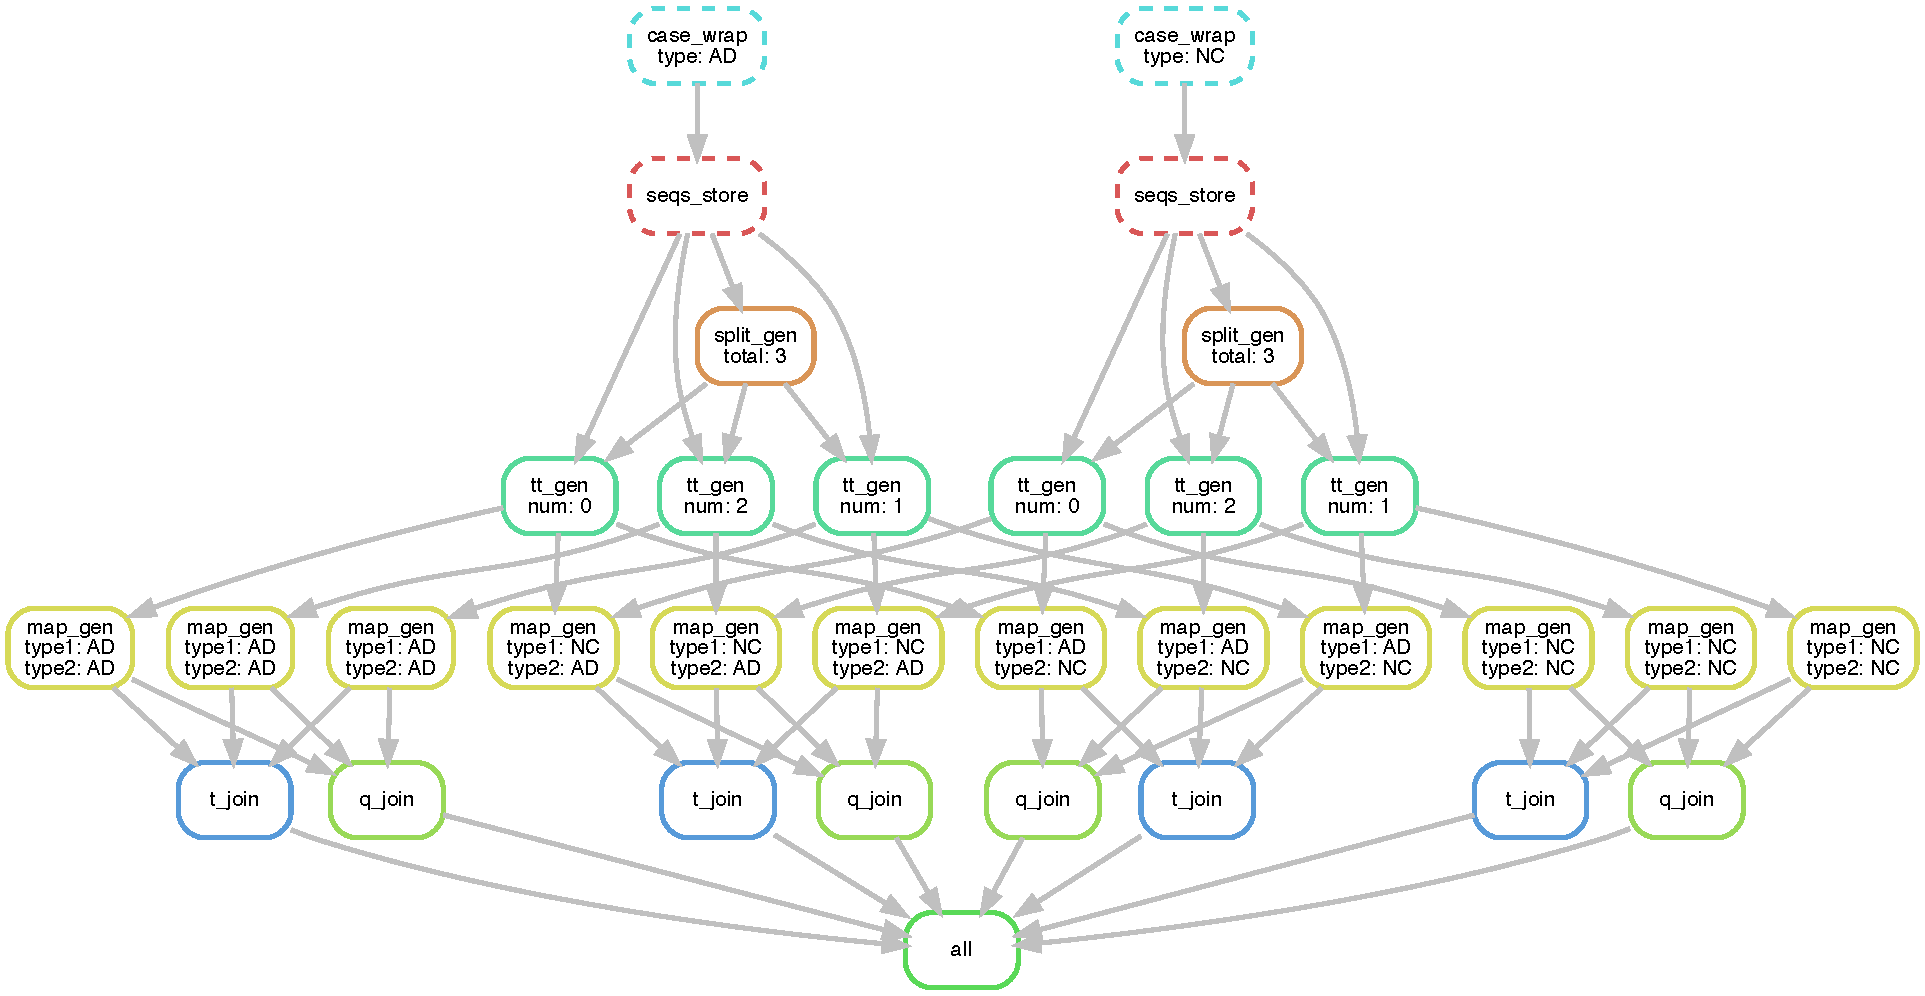
\includegraphics[scale=0.53, angle=270]{dag}
\caption{\textit{Directed Acyclic Graph representation of the WISDoM pipeline for the observations of ADNI database. Here we have 2 type of subject, labeled AD and NC, undergoing a 3 fold train-test split.}}
\label{dag}
\end{figure}

\subsection{Classification Methods}

The last steps of the pilenine are tied to clustering, classification and cross-validation on the dity dataset returned by the Snakemake section of the pipeline.

We now present a brief excursus on the methods used on the ADNI2 database.

Note that once the tidy dataset is obtained, a wide range of methods might be implemented in order to achieve clustering, classification, cross-validation and feature selection.

The methods we used are thus just a narrow selection of all the possibilities.

\subsection*{Hierachical Clustering}

In order to assess informations about classification performance and to find those feature whose weights are the most significant in assigning one element to a class or another, a \textit{hierchical clustermap} might be used as a fast and informative visualization.

The tool chosen is the \textit{clustermap} function of the \textit{Seaborn} \textit{python 3.6} module, as described in \textbf{seaborn.pydata.org/generated/seaborn.clustermap.html}.
\vspace{5mm}

As in \cite{cluster2}, hierarchical clustering's performances are \textit{metric} and \textit{linkage functions} dependent.

For the ADNI2 database clustering, metric used is a $L_1$ \textit{City Block}, defined as 
\begin{equation}
\sum_{j=1}^k \mid a_j - b_j \mid 
\label{mcl}
\end{equation}

between two $k$ dimensional points $a,b$. 

In this way, the effect of a large difference in a single dimension is dampened (since the distances are not squared) \cite{cluster}.

As far as linkage functions are concerned, we used a \textit{Nearest Point Algorithm}. 
\vspace{5mm}

Suppose there are $\mid u\mid$ original observations $(u[0],..., u[|u|-1])$ in cluster $u$ and $|v|$ original objects $(v[0], \ldots, v[|v|-1])$ in cluster $v$. Let $v$ be any remaining cluster in the forest that is not $u$.

The Nearest Point Algorithm assigns:

\begin{equation}
d(u,v) = \min(dist(u[i],v[j]))
\end{equation}

for all points $i$ in cluster $u$ and $j$ in cluster $v$.

Other possible linkage alghorithm are \cite{cluster2}:

\begin{itemize}
\item \textbf{Farthest Point Algorithm or Voor Hees Algorithm}, assigns:

\begin{equation}
d(u, v) = \max(dist(u[i],v[j]))
\end{equation}
for all points $i$ in cluster $u$ and $j$ in cluster $v$.

\item \textbf{UPGMA algorithm}, assigns:

\begin{equation}
d(u,v) = \sum_{ij} \frac{d(u[i], v[j])}{(|u|*|v|)}
\end{equation}

for all points $i,j$ where $|u|,|v|$ are the cardinalities of clusters $u,v$ respectively.

\end{itemize}

Further weighted methods are described in \cite{cluster2}.

\subsubsection*{Support Vector Machine Classification}

Another one of the methods used for classification and cross-validation is a classic \textit{Support Vector Machine}. The tool used is from the \textit{SKLearn Python 3.6} module.
More details can be found at:\\
 \textbf{scikit-learn.org/stable/modules/generated/sklearn.svm.SVC.html}
 
In general, a support vector machine can be seen as a generalization of linear decision boundaries for classification. 

In other terms, is a method to assess \textit{optimal separating hyperplanes} for non completely separable classes problems \cite{ESL}.
\vspace{5mm}

This is done by producing \textit{nonlinear boundaries} by constructing a linear boundary in a large, transformed version of the feature space.

An comparison of how a support vector classifier operates to solve non-separable problems is reported in fig.(\ref{svmc})
\clearpage

\begin{figure}[!h]
\centering
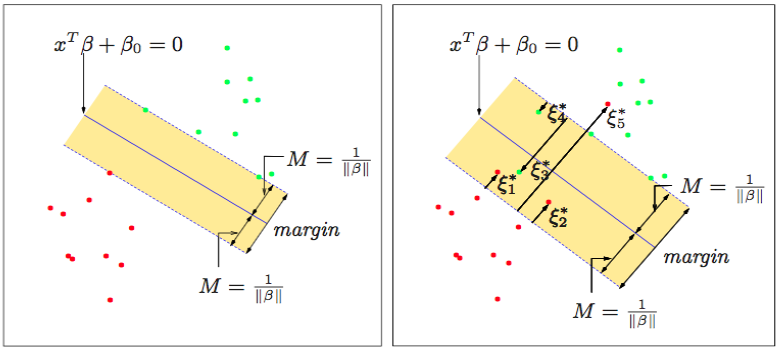
\includegraphics[scale=0.55]{svmc}
\caption{\textit{Support vector classifiers. The left panel shows the separable case. The decision boundary is the solid line, while broken lines bound the shaded maximal margin of width $2M=\frac{2}{||\beta ||}$.  The right panel shows the nonseparable (overlap) case. The points labeled $\xi^{\ast}_j$ are on the wrong side of their margin by an amount $\xi^{\ast}_j=M\xi_j$; points on the correct side have $\xi^{\ast}_j=0$. The margin is maximized subject to a total budget $\sum\xi_i\leq C$. Hence $\sum \xi^{\ast}_j$ is the total distance of points on the wrong side of their margin. \textbf{Source:} \textbf{Trevor Hastie, Robert Tibshirani, Jerome Friedman} \cite{ESL}. }}
\label{svmc}
\end{figure}

\subsubsection{Logistic Regression}

A method used to asses informative content of single features is the \textit{Logistic Regression}

Once again, a SKlearn Logistic Regression classifier is used. 
Details can be found at: \\ \textbf{scikit-learn.org/stable/modules/generated/sklearn.linear/}.
\vspace{5mm}

In general, the logistic regression model arises from the desire to model the posterior probabilities of the K classes via linear functions in $x$, while at the same time ensuring that they sum to one and remain in $[0,1]$.

When $K = 2$, this model is especially simple, since there is only a single linear function. It is widely used in biostatistical applications where binary responses (two classes) occur quite frequently \cite{ESL}.

The model has the form:

\begin{equation}
log\frac{p(G=(1,...,K-1)|X=x)}{p(G=k|X=x)}=\beta_{(1,...,K-1)0}+\beta^T_{(1,...,K-1)}x
\end{equation}

Logistic regression models are usually fit by maximum likelihood, using the conditional likelihood of $G$ given $X$. Since $p(G|X)$, $G=(1...,K-1,K)$ completely specifies the conditional distribution, the \textit{multinomial} distribution is appropriate. 

The log-likelihood for $N$ observations is:

\begin{equation}
l(\theta)=\sum_{i=1}^N log p_{gi}(x_i,\theta_i)
\end{equation}

where $p_k(x_i,\theta)=p(G = k|X = x_i; \theta)$.

\subsubsection{ROC AUC Score}

The score used to asses informative content and classification capabilities for each feature's logistic regression is the \textit{Receiver Operating Characteristic Area Under the Curve score}.

To grasp the meaning of the \textit{Receiving Operating Characteristic} score, we can think as follows. 

A ROC  curve is created by plotting the true positive rate (TPR) against the false positive rate (FPR) of a classifier at various threshold settings.

It is thus a plot of the \textit{sensitivity} (or \textit{probability of detection}) as a function of the \textit{fall-out} (or \textit{probability of false alarm}). 
\vspace{5mm}

Examples of ROC curves are reported in fig.(\ref{ADNI-roc}).

\begin{figure}[!h]
\centering
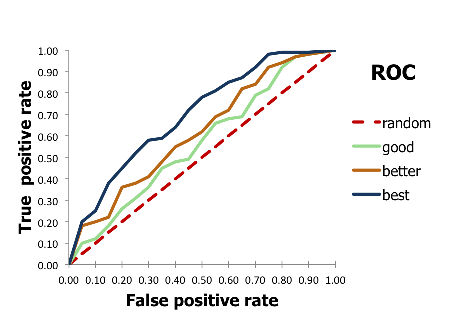
\includegraphics[scale=0.65]{roc-theory-small}
\caption{\textit{Sample ROC curves. A completely random classifier will migrate to the point $(0.5,0.5)$ while a perfect classification would be located at $(0,1)$.}
Credits: \textbf{https://docs.eyesopen.com/toolkits/cookbook/python/plotting/roc.html}}
\label{ADNI-roc}
\end{figure}

If the \textit{Area Under the Curve} is computed when using normalized units, we obtain a value tied to the informative power of a classifier, with a completely uninformative classifier (i.e a classifier based on completely random choices) yielding a value of $0.5$ \cite{ROC}.


\chapter{Results of The WISDoM Multiple Order Classification}

As stated in previous chapters, the chance to use the Wishart distribution to estimate covariance matrices distributions makes it extremely suitable for treating brain fMRI data and modelling problems.

Thus, to test WISDoM capabilities on feature selection and classification performances, two major databases of functional brain imaging data, the ADNI2 and ABIDE databases, have been explored and analyzed.

These two databases offer a good number of $p\times p$ \textit{correlation matrices}; one for each of the subjects that have undergone the baseline observations, as well as detailed labelling of different diagnostical groups.

The ADNI2 database contains observations about \textit{Alzheimer's disease} diagnoses and over-time conversions from \textit{mild cognitive impairment}, while the ABIDE study and database focuses on diagnostical groups of \textit{autism spectrum disorder}.
\vspace{5mm}

In both cases, data are fed to a WISDoM pipeline and a classification is attempted, while looking for the most significative features in classes' separation.

Furthermore, for comparison purposes, a class separation is attempted using a \textit{Network-Growth} method, while observing  the growth of random Wishart-generated networks in order to test the quality of the null-hypothesis.
\clearpage

\section{The ADNI2 Database: Study and Results}

ADNI, \textit{Alzheimer's Disease Neuroimaging Initiative}, is an ongoing, longitudinal, multicenter study designed to develop clinical, imaging, genetic, and biochemical biomarkers for the early detection and tracking of Alzheimer’s disease (AD). The ADNI study began in 2004 and included 400 subjects diagnosed with mild cognitive impairment (MCI), 200 subjects with early AD and 200 elderly control subjects.

The major goals of ADNI2 are to \cite{Adni}:

\begin{itemize}
\item Determine the relationships among clinical, imaging, genetic, and biochemical biomarker characteristics of the entire spectrum of Alzheimer’s Disease (AD), as the pathology evolves from normal aging through very mild symptoms, to mild cognitive impairment (MCI), to dementia.

\item Inform the neuroscience of AD, identify diagnostic and prognostic markers, identify outcome measures that can be used in clinical trials, and help develop the most effective clinical trial scenarios.

\item Develop improved methods which will lead to uniform standards for acquiring longitudinal multi-site MRI and PET data on patients with AD, MCI, and elderly controls.

\item Perform longitudinal clinical, cognitive, MRI, PET (18F-AV-45 and
FDG), and blood and CSF biomarker studies on 550 newly enrolled
subjects in four diagnostic categories – cognitively normal (CN),
early MCI (EMCI), late MCI (LMCI), and mild AD. 

\item Collect blood samples for DNA and RNA extraction. Newly enrolled subjects will also have samples collected for Cell Immortalization and APOE genotyping.

\item Validate the clinical diagnoses and imaging and biomarker surrogates through neuropathological examination of ADNI1, GO and ADNI2 participants who come to autopsy.

\end{itemize}

A resume of how the clicnical data are collected for 54 months after the baseline is reported in fig. (\ref{clinicADNI})

\clearpage

\begin{figure}[!h]
\centering
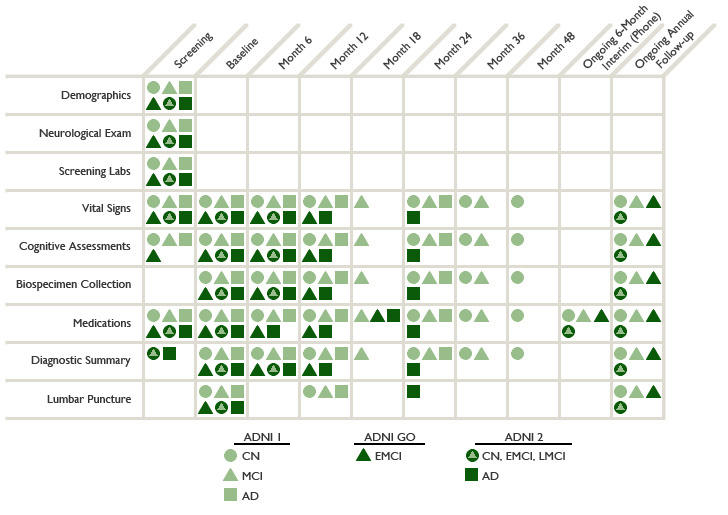
\includegraphics[scale=0.5]{clinical-ADNI}
\caption{\textit{Timeline of clinical data collection procedures. Source: \textbf{http://adni.loni.usc.edu/data-samples/clinical-data/}}}
\label{clinicADNI}
\end{figure}

\subsection{Data Exploration and Selection for WISDoM Classification}

As a preliminar analysis, the conversion rate of MCI to AD has been checked in order to find correspondence with literature. As in \cite{conv}, \cite{conv2} , we expect to find a maximum of the conversions' distribution over time at around 18 months. 

This period of time is, as a matter of fact, the cut-off for what has been defined \textit{long-term survival}, after which prediction results for conversion significantly lose stability \cite{conv2}.

As shown in figure (\ref{conv-comp}), the maximum for the distribution stands at around 18 months.

Two different fits are reported for comparison in terms of log-likelihood.

\begin{figure}[!h]
\centering
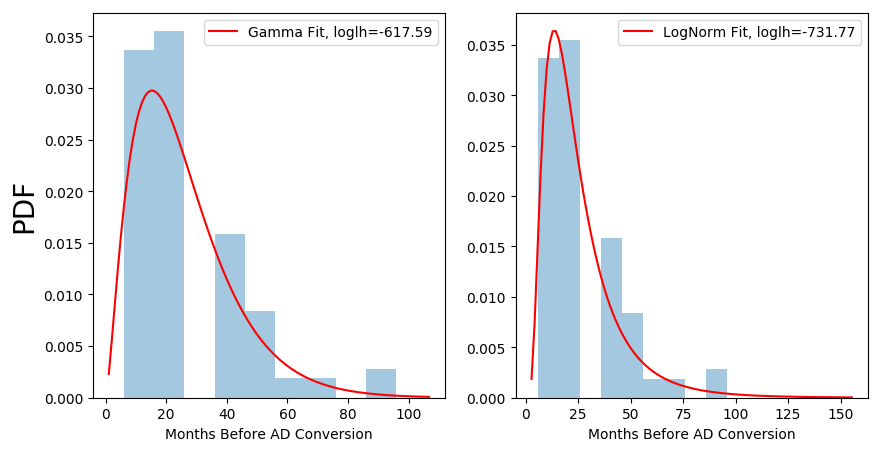
\includegraphics[scale=0.65]{conv-comp}
\caption{\textit{Conversion distribution over time. As expected, we find a maximum at around 18 months. Two different fits (Gamma and Log-normal) are reported for comparison.}}
\label{conv-comp}
\end{figure}

\vspace{5mm}

Of the 403 total subjects available, only 232 were selected for the final WISDoM Classification run.

The main reason of such a selection is the fact that two distinct data group can be found inside the datasets.

As shown in fig.(\ref{std-ADNI}), two distinct peaks are obtained if a standard deviation distribution for the diagnostic groups is taken into account.

While no difference in distribution can be found amongst the three different diagnostic grups, the second peak can be a sign of two indipendent data normalization procedures in the dataset.

To support this hypothesis, if we look at the standard deviation distribution by gender in fig.(\ref{std-gen-ADNI}), we can see that there are two different gender labelling (M-F and Male-Female) generating two distinct peaks. 

This fact leads to the hypothesis that two distinct datasets, whos subjects have been examined with silghtly different procedures, might have been merged into a single one.

\begin{figure}[!h]
\centering
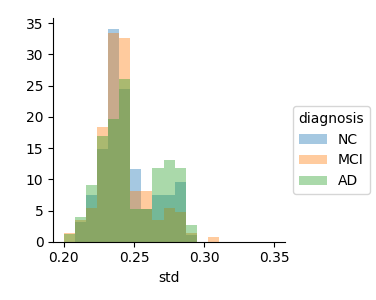
\includegraphics[scale=0.75]{std-ADNI}
\caption{\textit{Standard deviation for different diagnostic groups. As shown, different diagnostic groups yields no signficative difference while the second peak at $\sim 0.27$ might be due to different normalizations in data.}}
\label{std-ADNI}
\end{figure}

\begin{figure}[!h]
\centering
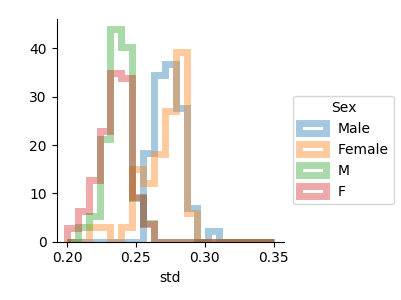
\includegraphics[scale=0.75]{ADNi-std-gen}
\caption{\textit{Standard deviation distribution by gender. The two distinct peak are a sign of different normalization for data whose gender is labelled with M-F and Male-Female.}}
\label{std-gen-ADNI}
\end{figure}

Given that the Male-Female labelling occurs for the first 98 entries, the remaining 305 entries have been chosen for the final run, being the biggest group with homogeneous data normalization.

Of these 305 entries, 7 have been discarded due to wrong or missing labelling.

Of the remaining entries, subjects of the \textit{Mild Cognitive Impairment (MCI)} diganostic group have been excluded.

This choice has been made in order to train the classifier exclusively on the \textit{Normal Control (NC)} group, and \textit{Alzheimer's Disease (AD)} diagnostic groups.

In this way, the conversion component is excluded form the analysis, whose aim is to classify and select significative features for the NC and AD diagnostic groups.

Of the 232 subjects remaninig, the 63\% belongs to diagnostic group AD and the remaining 37\% belongs to diagnostic group NC.

\subsubsection*{Data Structure and Preprocessing}

Each subject's image has been preprocessed and divided into 549 \textit{macrovoxels}, whose \textit{topological correlation} has been computed with respect to each other, each of the 549 macrovoxels being defined over an ensemble of $3 \cdot 10^3$ voxels.

Thus, 232 $N\times N$ , $N=549$ matrices have been used for training and calssification with the WISDoM classifier.

An example of such a corelation matrix can be seen in fig.(\ref{sample-heat}).

\begin{figure}[!h]
\centering
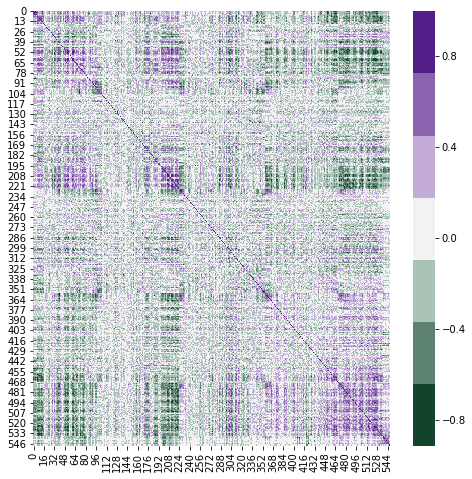
\includegraphics[scale=0.5]{sample-heat}
\caption{\textit{Divergent heatmap representation of a subject's correlation matrix.}}
\label{sample-heat}
\end{figure}

\subsection{Results}

Several types of analyses and classifications have been conducted on the outputs of the WISDoM method's  features transformations defined in eq.(\ref{pdf-score}), eq.(\ref{JSscore}) and eq.(\ref{JRatio}).

First of all, a separation of the two classes AD and NC based on complete matrix distance (eq.(\ref{pdf-score})) is attempted.

Then, single feature distances as in eq.(\ref{JSscore}, \ref{JRatio}) are computed for all the subjects and various clusterings and calssifications are attempted.

Lastly, a network-growth separation based on transformed features ranking is attempted for comparison.

\subsubsection*{Complete Matrix Distance Separation}

As a first approach to classification, a score based on simple log-likelihood distance is assigned to each subject's correlation matrix. In fig.(\ref{ADNI-global}) is reported the attempt to separate the two diagnostic groups AD and NC by computing the distance in terms of log-likelihood from each class's estimated Wishart distribution.

As seen before, one class's WIshart distribution can be estimate by computing the scale matrix as in eq.(\ref{Class-Scale}). 

In this case the parameter \textit{degrees of freedom} $n$ is given by the number of voxels belonging to each macrovoxel. Thus, we take $n=3\cdot 10^3$.

\begin{figure}[!h]
\centering
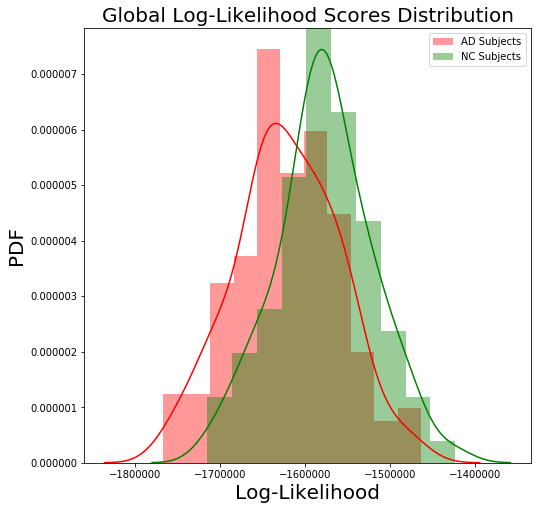
\includegraphics[scale=0.5]{ADNI-global}
\caption{\textit{Complete matrix log-likelihood score distribution, separation performance is abysmal.}}
\label{ADNI-global}
\end{figure}

Then, a \textit{complete matrix ratio score} as in eq.(\ref{pdf-score}) is assigned to each matrix for classifficiation. 

Results for this type of process are shown in fig.(\ref{ADNI-Rglobal}).

\begin{figure}[!h]
\centering
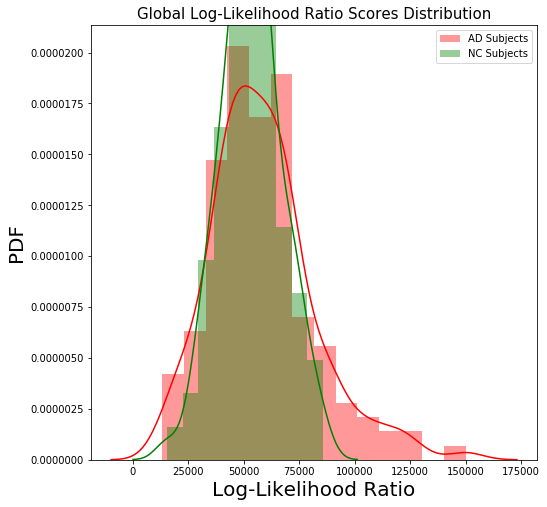
\includegraphics[scale=0.5]{ADNI-Rglobal}
\caption{\textit{Complete matrix log-likelihood ratio score distribution, separation performance is abysmal.}}
\label{ADNI-Rglobal}
\end{figure}

At this stage, it is clear that separation performances are inadequate and single feature analysis is needed.

\subsubsection{Single Feature Ratio Separation}

For each one of the 232 subject, the $(p-1)$ order feature transformation is computed according to eq.(\ref{JSscore}); this is done thanks to the WISDoM Classification pipeline described by figure (\ref{gpipe}).

We set the pipeline to compute the estimated Wishart distribution for the classes from each train batch in a \textit{10-fold cross validation process}; test elements' feature are then transformed and the score vector for order $(p-1)$ transformation is computed.

This leads to a $90\%-10\%$  \textit{train-test splitting} for each batch.

After the score vector is computed with respect to each class for each subject, scores defined by eq.(\ref{JRatio}) are computed and the vectors merged into a single tidy dataset.

Various classification processes are then attempted.
\vspace{5mm}

To compare separation performances after single feature analysis, in a way similar to what has been done for complete matrix distance separation described in fig.(\ref{ADNI-global}, \ref{ADNI-Rglobal}), the distribution of single scores assigned for each subject is computed.

This is simply done via a sum of the single feature ratio score vector for each subject. 

Results can be seen in fig.(\ref{ADNI-sfsum}).

\begin{figure}[!h]
\centering
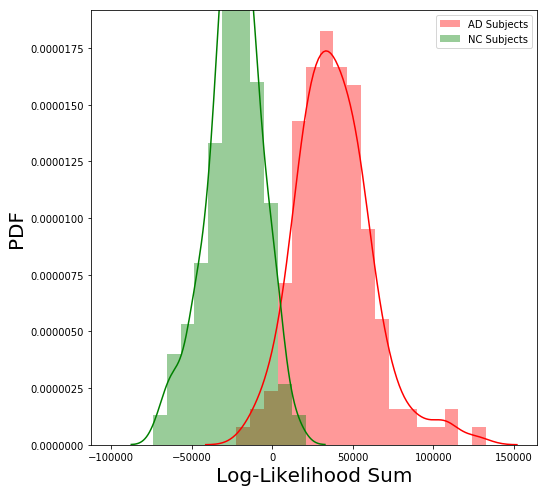
\includegraphics[scale=0.5]{diff-logpdf-dist}
\caption{\textit{Distribution of the sums of single feature ratio score vector for each subject. In this way, a vector of scores is reduced to a single score. Looking at the distributions we can see that classes are already well separated with this simple reduction.}}
\label{ADNI-sfsum}
\end{figure}

Comparing the results shown in fig.(\ref{ADNI-sfsum}) with the results for complete matrix disatnce separation in fig.(\ref{ADNI-global}, \ref{ADNI-Rglobal}), we can state that the $(p-1)$ order feature transformation and ratio score already give a significant separation perfomance enhancement at this stage.

\subsubsection*{Clustering}

In order to obtain information about which features are the most significative in classification, a \textit{hierachical clustering}, described in \cite{cluster}, \cite{cluster2},  is performed.
\vspace{5mm}

Such a clustermap, shown in fig.(\ref{ADNI-cluster}), offers a representation of the classification capabilities and weights of single features.

As a matter of facts, features on the left part of the map are seen as the most significative in clustering performance.

We can also state that a clustering made on $(p-1)$ order transformed features yields a good performance for the groups NC (in green) and AD (in red). Only a few subjects tends to be assigned to clusters far from their true classes' main clusters.

\begin{figure}[!h]
\centering
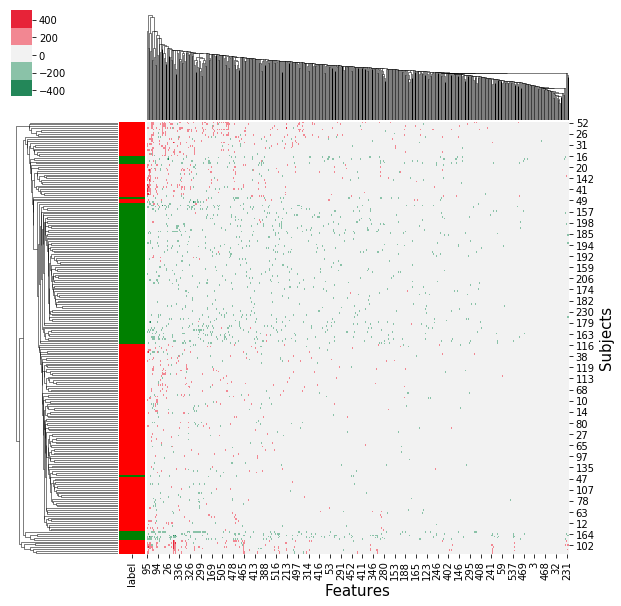
\includegraphics[scale=0.5]{diff-logpdf-clustering10}
\caption{\textit{Hierarchical Clustering visualization over an $L_1$ City Block Metric. Features on the left part of the map have the biggest influence in clustering decision. Color green is assigned for NC subjects and red for AD subjects.}}
\label{ADNI-cluster}
\end{figure}

\subsubsection*{SVM Classification and Single Feature Logistic Regression Ranking}

Given the results obtained with scores' sum distributions and clustering, a classification with a \textit{C-Support Vector Machine} has been attempted. 

Using a linear kernel and taking the penalty parameter for error term $C=1$, a \textit{10 fold stratified cross-validation} is performed.

Note that the use of  a stratified cross-validation means that the relative proportions of the classes are preserved for each train-test batch, as in \cite{ESL}.

Such a classification yields  an\textit{ accuracy score} of $100\%$.
\vspace{5mm}

Again, given the results, a \textit{single feature logistic regression classifier} has been tested, in order to observe each feature classification performances and produce a feature ranking.

This is done by computing a logistic regression classification for each one of the 549 transformed features of each subject and computing the average cross-validation \textit{ROC AUC} score for each feature.

At this stage, a logistic regression classification is attempted using a single feature for each iteration.

Then a 10-folds cross validation is computed and the average ROC AUC score is assigned to each feature, as an indicator of classification performance.

A plot of the  classification capabilities, in terms of ROC AUC score, over features' ranking is reported in fig.(\ref{ADNI-frank}). 

\begin{figure}[!h]
\centering
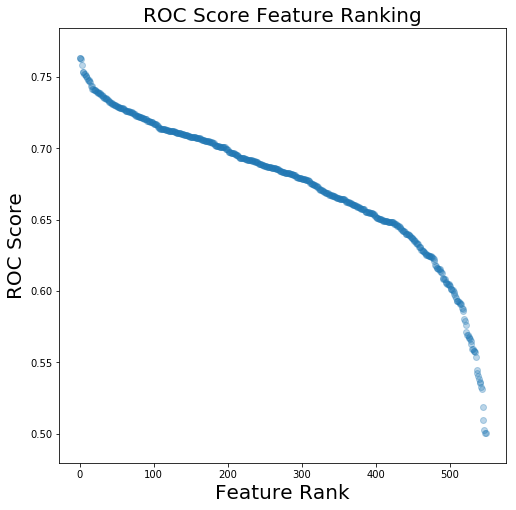
\includegraphics[scale=0.5]{ROC-feature-rank}
\caption{\textit{ROC score over ranking. Note that by definition a ROC score of 0.5 means a completely random classification. We can see that classification capabilities rapidly decrease after the first 300 rankings.}}
\label{ADNI-frank}
\end{figure}

If the \textit{Area Under the Curve} is computed when using normalized units, we obtain a value tied to the informative power of a classifier, with a completely uninformative classifier (i.e a classifier based on completely random choices) yielding a value of $0.5$ \cite{ROC}.
\vspace{5mm}

Thus, computing a regression for each feature and the relative ROC AUC score will tell how informative a classifier based on that single feature is. 

To visualize he informative content of the highest ranking features and take a look at their classification capabilities, we attempted to separate the two classes in the first two highest ranked features' space.

Beside scattering each class's elements, a linear regression for each class is plotted.

Results are shown in fig.(\ref{ADNI-fsep}).

\begin{figure}[!h]
\centering
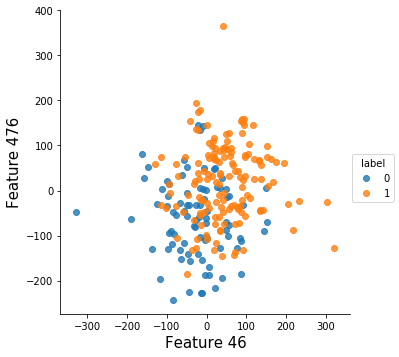
\includegraphics[scale=0.7]{first-feat-sep}
\caption{\textit{Scatterplot in the first two highest ranked features' space. While  the elements of each class are far from being completely separate, we can see that the regressions computed for each one of the classes are not overlapping, even if a confidence interval is plotted. Label 1 is assigned to class AD while label 0 is assigned to class NC. }}
\label{ADNI-fsep}
\end{figure}

While the separation is obviously not comparable to results obtained and shown by fig.(\ref{ADNI-sfsum}) or fig.(\ref{ADNI-cluster}), we can state that reducing the classification to the first two highest features (in other terms, reducing the problem to two dimensions) doesn't cause the classification to be completely uninformative.

As a matter of fact, we can see that the simple regressions shown in fig.(\ref{ADNI-fsep}) already mantain a disctinct trend.

\subsubsection*{Network Growth Separation for Non-Transformed Features}

In order to emphasize the importance of the features' transformation defined in eqs.(\ref{JSscore}, \ref{JRatio}) in classification performance enhancement, we attempted to obtain some separation results on non.transformed features via a \textit{threshold-based network growth} process.
\vspace{5mm}

First, all matrices have been standardized. Then a ranking of absolute correlation values is made, in order to obtain a \textit{sorted edges list} upon which the networks' growth is based and nodes are created.

At this point, a network is observed in terms of \textit{number of nodes}, \textit{number of connected components}, \textit{size of the biggest connected component} while adding an edge for each iterations. 

In this way, the strongest connections in terms of correlations between features are the first to generate nodes in the network for each iterations. The goal is to establish if Alzheimer's diagnosed subjects network of correlations grows at a slower rate than normal control subjects' networks.

Each network's growth is observed for a range of $3\cdot 10^3$ edges.

Besides observing networks for the two diagnostical groups AD and NC,  growth of \textit{Erdos-Reniy} random networks and \textit{Random Wishart sampled} networks is also reported for comaprison. Results are shown in fig.(\ref{ADNI-Ngrowth}).

The Wishart random sampling networks are generated using the \textit{average of all ADNI2's subjects matrices as the scale matrix}.
\vspace{5mm}

By looking at fig.(\ref{ADNI-Ngrowth}), we see that no significative separation is shown for the two classes.

On the other side, we can see that the growth trend of Wishart-generated random networks is comparable with that of real AD and NC observations, thus validating the model used for the generation of the estimated distributions.

\begin{figure}[!h]
\centering
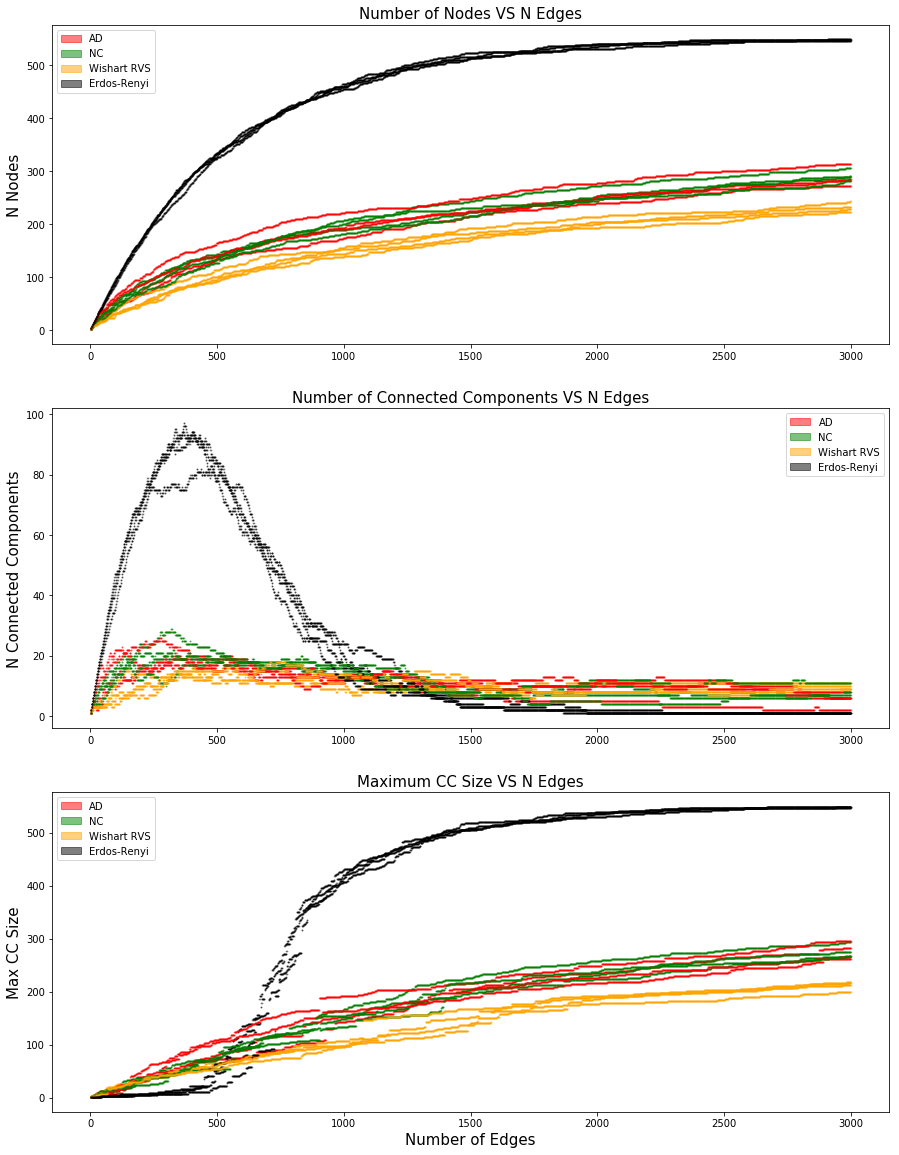
\includegraphics[scale=0.5]{ADNI-Ngrowth}
\caption{\textit{Networks growth observed in terms of Number of Nodes, Number of Connected Components and Size of largest Connected components. 4 subjects are plotted for each category in order to give an idea of variability. While separation performances are abysmal, we can see that the Wishart null hypothesis is well suited, as its trend is comparable with AD and NC subjects' trend. }}
\label{ADNI-Ngrowth}
\end{figure}

\clearpage

To get a more accurate idea of inter-class growth's average behaviour, a \textit{Lowess Regression} \cite{Lowess} as been computed on \textit{50} subjects for each of the diagnostic group AD and NC.

As shown in fig.(\ref{ADNI-lowess}), there is no significative separation between the two classes.

An issue with fig.(\ref{ADNI-lowess}) is that the tool used to compute the lowess did not allow the visualization of a confidence interval; we can see however that regression's lines are overlapping even without a confidence inerval. 

\begin{figure}[!h]
\centering
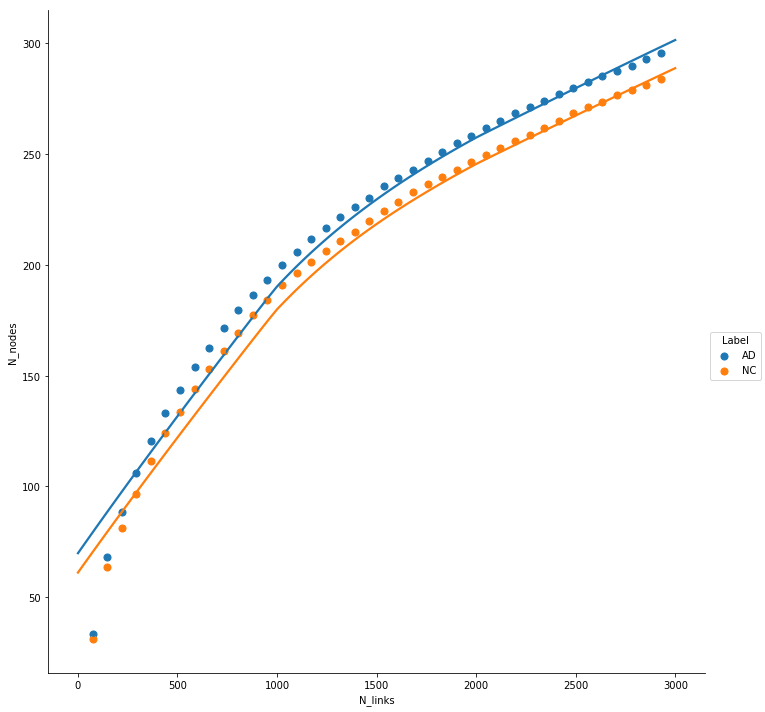
\includegraphics[scale=0.4]{ADNI-lowess}
\caption{\textit{Lowess regression on 50 subjects-per-class growth. No significant separation is yielded, given that for the tool used, a confidence interval for the plot could not be visualized. The x axis has been binned into 40 values to enhance visualization.}}
\label{ADNI-lowess}
\end{figure}

\chapter*{Conclusions}

\backmatter

\begin{thebibliography}{99}

\bibitem{Neuro-Hist}
Randy L. Buckner, Jessica R. Adrews-Hannaand Daniel L. Schacter

\emph{The Brain’s Default Network Anatomy, Function, and Relevance to Disease}

New York Academy of Sciences 2008

\bibitem{default-mode}
Raichle M. E., MacLeod A. M., Snyder A. Z., Powers W. J., Gusnard D. A., and Shulman G. L.

\emph{A Default Mode of Brain Function}

Proceedings of the National Academy of Sciences, 98 (2), pp. 676-682, 2001

\bibitem{DMN}
Fox M. D., Snyder A. Z., Vincent J. L., Corbetta M., Van Essen D. C., and Raichle M. E.

\emph{The Human Brain is Intrinsically Organized into Dynamic, Anticorrelated Functional Networks}

Proceedings of the National Academy of Sciences, 102, pp. 9673-9678, 2005

\bibitem{RNS}
M. P. Van Den Heuvel and H. E. H. Pol.

\emph{Exploring the Brain Network: a Review on Resting-State fMRI Functional Connectivity}

European Neuropsychopharmacology, 20(8):519–534, 2010

\bibitem{Rest-NTW}
E. Bullmore and O. Sporns

\emph{ Complex brain networks: graph theoretical analysis of structural and functional systems}

 Nature Reviews Neuroscience, 10(3):186–198, 2009.

\bibitem{ssa}
Xiaohu Zhao , Yong Liu , Xiangbin Wang, Bing Liu, Qian Xi, Qihao Guo, Hong Jiang, Tianzi Jiang , Peijun Wang 

\emph{Disrupted Small-World Brain Networks in Moderate Alzheimer's Disease: A Resting-State fMRI Study}

March 23, 2012

DOi: https://doi.org/10.1371/journal.pone.0033540

\bibitem{bold}
N. K. Logothetis

\emph{ What we Can Do and What we Cannot Do with fMRI}

Nature, 453(7197):869–878, 2008.

\bibitem{atlas}
A. C. Evans, D. L. Collins, S. Mills, E. Brown, R. Kelly, and T. M. Peters.

\emph{3d Statistical Neuroanatomical Models from 305 MRI Volumes}

In Nuclear Science Symposium and Medical Imaging Conference, 1993., 1993 IEEE Conference Record.,

pages 1813–1817. IEEE, 1993.

\bibitem{connect}
Friston

\emph{Functional and Effective Connectivity: A Review}

 Brain Connectivity, 1, 13-36, 2011

\bibitem {AMS}
Hardle, Wolfgang and Leopold Simar

\emph{Applied Multivariate Statistical Analysis}

Heidelberg: Springer Berlin Heidelberg, 2012

\bibitem {IMS}
Anderson, T. W.

\emph{An Introduction to Multivariate Statistical Analysis}
 
New York: John Wiley and Sons,  2003

\bibitem{SML}
 Han Liu and Larry Wasserman
 
 \emph{Statistical Machine Learning}

 Pittsburgh: CMU University, 2014
 
\bibitem{CBA}
Murphy, Kevin P.

\emph{Conjugate Bayesian Analysis of the Gaussian Distribution}

Vancouver: University of British Columbia, 2007
 
\bibitem{WishGen}
W.B. Smith and R.R. Hocking

\emph{Algorithm AS 53: Wishart Variate Generator}

Applied Statistics, vol. 21, pp. 341-345, 1972.

\bibitem{SnakeMake}
Köster, Johannes and Rahmann, Sven

\emph{Snakemake - A scalable bioinformatics workflow engine}

Bioinformatics, Volume 28, Issue 19, Pages 2520–2522,1 October 2012

DOI: https://doi.org/10.1093/bioinformatics/bts480

\bibitem{Adni}
ADNI Commitee

\emph{Alzheimer's Disease Neuroimaging Initiative - Procedures Manual}

http://adni.loni.usc.edu/, January 2016


\bibitem{conv}
Ke Liu, Kewei Chen, Li Yao and Xiaojuan Guo

\emph{Prediction of Mild Cognitive Impairment Conversion Using a Combination of Independent Component Analysis and the Cox Model}

Frontiers in Human Neuroscience, 06 February 2017

DOI:  https://doi.org/10.3389/fnhum.2017.00033

\bibitem{conv2}
Wei R., Li C., Fogelson N., Li L.

\emph{Prediction of Conversion from Mild Cognitive Impairment to Alzheimer's Disease Using MRI and Structural Network Features}

Frontiers in Aging Neuroscience  19 April 2017

DOI: 10.3389/fnagi.2016.00076

\bibitem{cluster}
Ziv Bar-Joseph, David K. Gifford, Tommi S. Jaakkola, 

\emph{Fast Optimal Leaf Ordering for Hierarchical Clustering}

 Bioinformatics, 1 June 2001
 
 DOI: https://doi.org/10.1093/bioinformatics/17.suppl\_1.S22
 
\bibitem{cluster2}
 Daniel Mullner
 
\emph{Modern Hierarchical, Agglomerative Clustering Algorithms} 

12 September 2011

DOI: https://arxiv.org/abs/1109.2378v1

\bibitem{ESL}
Trevor Hastie, Robert Tibshirani, Jerome Friedman

\emph{The Elements of Statistical Learning}

Springer ISBN 978-0-387-84858-7

\bibitem{ROC}
Hand, David J. and Till, Robert J.

\emph{A simple generalization of the area under the ROC curve for multiple class classification problems,}

Machine Learning, 45, 2001

\bibitem{Lowess}
Cleveland, W.S. 

\emph{Robust Locally Weighted Regression and Smoothing Scatterplots}

Journal of the American Statistical Association 74 (368): 829-836, 1979



 \end{thebibliography}
 
 
\end{document}